%===========================================================
%== Präambel ===============================================
%===========================================================
\documentclass[
    paper=a4,
    bibtotocnumbered,
    liststotocnumbered,
    oneside,
    12pt,
    listof=totoc,
    toc=chapterentrywithdots,
    listof=entryprefix,
]{scrreprt}

\usepackage[a4paper, left=2.5cm, right=2.5cm, top=1.25cm, bottom=1.25cm, includehead, includefoot]{geometry}


\usepackage{float}
\usepackage[T1]{fontenc}%Encoding
\usepackage[german]{babel}%German-specific commmands
%\usepackage[utf8]{inputenc} %Wird nicht benötigt bei XeLatex
\usepackage{fancyhdr}%% Kopfzeile u. Fußzeile
\usepackage{fontspec}%% Schriftart
\usepackage[onehalfspacing]{setspace}%-- Zeilenabstand 1,5
\usepackage[toc, nopostdot, acronyms, nonumberlist]{glossaries}%% Glossar
\usepackage[intoc]{nomencl}%% Symbolverzeichnis
\usepackage{etoolbox}%Sorgt dafür, das Symbolverzeichnis im Header steht
\usepackage[]{minted}
\usepackage[titles]{tocloft}
\usepackage{scrhack}
\usepackage{colortbl}%Einfärben von Tabellen-Zellen, Zeilen, Spalten
\usepackage[]{layout}
\usepackage[]{blindtext}
%\usepackage{showframe}% zum Anzeigen des Seitenlayouts
\usepackage[figurename={Abb.},tablename={Tab.}]{caption}%Anpassung der Namen für Abbildung und Tabelle
\usepackage[]{url}
\usepackage[]{hyperref}
\usepackage{chngcntr}%% Nummerierung der Abbildungen und Tabellen fortlaufend %%%%%%
\usepackage{tocbibind}
\usepackage[style=alphabetic, citestyle=alphabetic, ,maxcitenames=1,uniquelist=false]{biblatex}
\usepackage[babel,german=quotes]{csquotes} % Deutsche
\usepackage{booktabs}
\usepackage[final]{showkeys}
\usepackage{tabularx}
\usepackage{tabulary}

\usepackage{etoolbox}
\BeforeBeginEnvironment{listing}{\vspace{0cm}}
\AfterEndEnvironment{listing}{\vspace{-0.5cm}}
\BeforeBeginEnvironment{minted}{\vspace{-0.3cm}}
\AfterEndEnvironment{minted}{\vspace{-0.3cm}}
\BeforeBeginEnvironment{quote}{\vspace{-0.1cm}}
\AfterEndEnvironment{quote}{\vspace{-0.1cm}}

% Paragraph styles
\setlength{\parindent}{0cm}
\setlength{\parskip}{6pt}

%% Kopfzeile u. Fußzeile
\pagestyle{fancy}
\fancyfoot{}
\fancyfoot[R]{\thepage}
\fancyhead{}
\fancyhead[L]{\nouppercase{\leftmark}}
\fancypagestyle{plain}{\pagestyle{fancy}}


%-- Standardschriftart auf Times New Roman umstellen
\setmainfont[ Path = Fonts/,
BoldFont=timesbd.ttf,
ItalicFont=timesi.ttf,
BoldItalicFont=timesbi.ttf
]{times.ttf}

%-- Kapitelüberschriften auf Standardschriftart(Times New Roman) umstellen
\setkomafont{disposition}{\normalcolor\bfseries}

% Entfernt "Kapitel X" aus der Kopfzeile vor der Kapitelüberschrift
\renewcommand{\chaptermark}[1]{\markboth{\MakeUppercase{#1}}{}}
 
%Abstände nach Kapiteln 
\RedeclareSectionCommand[%
  beforeskip=0pt,
  afterskip=1\baselineskip plus .1\baselineskip minus .167\baselineskip
]{chapter}

%% Nummerierung der Abbildungen und Tabellen fortlaufend %%%%%%
\counterwithout{figure}{chapter}
\counterwithout{table}{chapter}

%% Rahmen in Textbreite um Bilder
\floatstyle{boxed}
\restylefloat{figure}
%\restylefloat{table}
\restylefloat{listing}

%% Captions linksbündig orientieren
\captionsetup{justification=raggedright,singlelinecheck=false}

% Einbinden von Glossar u. Abkürzungsverzeichnis
%-----------------------------------------------------------------------------
% Glossar
%-----------------------------------------------------------------------------

% \newglossaryentry{Literal}
% {
%     name=Literal,
%     description={\todo{Was ist ein Literal}}
% }
\input{Verzeichnisse/Abkürzungsverzeichnis.tex}
\makeglossaries

% Hinzufügen von Bib-Dateien
\addbibresource{Literatur/literatur.bib}

\newminted[GoCode]{go}{linenos=true, xleftmargin=.7cm, fontsize=\small}
\newminted[SwiftCode]{swift}{linenos=true, xleftmargin=.7cm, fontsize=\small}
\newmintedfile[InputGo]{go}{linenos=true, xleftmargin=.7cm, fontsize=\small}
\newmintedfile[InputSwift]{swift}{linenos=true, xleftmargin=.7cm, fontsize=\small}
\newminted[Commandline]{bash}{linenos=true, xleftmargin=.7cm, fontsize=\small}

\usepackage{color}
\newcommand{\todo}[1]{\textcolor{white}{\colorbox{red}{ To do %
      :}}\textcolor{red}{\ \ #1
  }\textcolor{red}{\colorbox{red}{III}}\ }


\def\listingautorefname{Codebeispiel}% 

\newcolumntype{L}[1]{>{\raggedright\arraybackslash}p{#1}} % linksbündig mit Breitenangabe
\newcolumntype{C}[1]{>{\centering\arraybackslash}p{#1}} % zentriert mit Breitenangabe
\newcolumntype{R}[1]{>{\raggedleft\arraybackslash}p{#1}} % rechtsbündig mit Breitenangabe


\newcommand{\dummyfig}[1]{
  \centering
  \fbox{
    \begin{minipage}[c][0.33\textheight][c]{0.5\textwidth}
      \centering{#1}
    \end{minipage}
  }
}

\definecolor{Gray}{gray}{0.75}
\definecolor{lightblue}{rgb}{0.93,0.95,1.0}




\begin{document}

%===========================================================
%== Titelseite =============================================
%===========================================================
\newgeometry{left=2.5cm, right=2.5cm, top=2.5cm, bottom=2.5cm}
\begin{titlepage}
    \begin{center}
    
\includegraphics[width=\textwidth]{Images/logo}
        \begin{Large}
        Hochschule für angewandte Wissenschaften Coburg
        \\
        Fakultät Elektrotechnik und Informatik
        \par
        \end{Large}
        \vspace{2.0cm}
        
        \begin{Large}
            Studiengang: Informatik
            \par
        \end{Large}
        \vspace{1.5cm}
        
        {\Large
            Bachelorarbeit
        }
        \vspace{2.0cm}

        \begin{huge}
            \textbf{Vergleich von Google Go und Apple Swift} 
            \par
        \end{huge}        
        \vfill
        
        \begin{huge}
            Daniel Müller
        \end{huge}
        \vspace{2.0cm}
        
        \begin{large}
            Abgabe der Arbeit: 08. Juni 2017
            
            Betreut durch:
            \\
            Prof. Volkhard Pfeiffer, Hochschule Coburg
            \\
            %<optional: Zweitgutachter: Prof. Dr. XXX, Hochschule Coburg>
            \par
        \end{large}
        
    \end{center}
\end{titlepage}
\restoregeometry

%===========================================================
%== Abstract ===============================================
%===========================================================
\begin{abstract}
    Die vorliegende Bachelorarbeit ist ein Vergleich der beiden Programmiersprachen Go und Swift.
    Zu diesem Zweck werden unterschiedliche Kriterien aufgestellt, anhand derer die beiden Programmiersprachen miteinander verglichen werden. 
    Der Vergleich soll klären, inwiefern Go und Swift Gemeinsamkeiten aufweisen und welche Unterschiede zwischen Go und Swift bestehen.
\end{abstract}

\begin{abstract}
    The goal of this paper is to compare Go and Swift.
    To aim this goal, different criterias are established to compare these programming languages.
    This Comparsion is about finding similarities and showing differences of Go and Swift.
\end{abstract}
    
%===========================================================
%== Inhaltsverzeichnis =====================================
%===========================================================   
\begin{singlespace}
\renewcommand{\cftchapleader}{\cftdotfill{\cftdotsep}} % Punkte im Inhaltsverzeichnis bei Kapiteln
\tableofcontents
\end{singlespace}

%===========================================================
%== Abbildungsverzeichnis ==================================
%===========================================================
\newpage
\renewcommand{\cftfigpresnum}{Abb. }
\renewcommand{\cftfigaftersnum}{:}
\setlength{\cftfignumwidth}{2cm}
\setlength{\cftfigindent}{0cm}
\listoffigures

%===========================================================
%== Tabellenverzeichnis ====================================
%===========================================================
\newpage
\renewcommand{\cfttabpresnum}{Tab. }
\renewcommand{\cfttabaftersnum}{:}
\setlength{\cfttabnumwidth}{2cm}
\setlength{\cfttabindent}{0cm}
\listoftables

%===========================================================
%== Codeverzeichnis ========================================
%===========================================================
\newpage
\renewcommand\listingscaption{Code}
\renewcommand\listoflistingscaption{Codebeispielverzeichnis}
\renewcommand{\cftfigpresnum}{Code }
\listoflistings
\addcontentsline{toc}{chapter}{Codebeispielverzeichnis}

% %===========================================================
% %== Symbolverzeichnis ======================================
% %===========================================================
% \newpage
% %% Symbolverzeichnis
% \makenomenclature
% % This will add the units
% %----------------------------------------------
% \newcommand{\nomunit}[1]{%
% \renewcommand{\nomentryend}{\hspace*{\fill}#1}}
% %----------------------------------------------
% \renewcommand{\nomname}{Symbolverzeichnis}
% %Sorgt dafür, das Symbolverzeichnis im Header steht
% \patchcmd{\thenomenclature}
%   {\chapter*{\nomname}}% usually only \chapter*{\nomname} is issued
%   {\chapter*{\nomname}\markboth{\MakeUppercase\nomname}{\MakeUppercase\nomname}}
%   {}{}
% %-----------------------------------------------------------------------------------
% Symbolverzeichnis
%-----------------------------------------------------------------------------------
% Bsp: \nomenclature[prefix]{symbol}{description}

\nomenclature[]{$c$}{Speed of light in a vacuum inertial system \nomunit{$299,792,458\, m/s$}}

\nomenclature[]{$i$}{Ganzzahlige Laufvariable \nomunit{Integer}}
% \printnomenclature


%===========================================================
%== Abkürzungsverzeichnis ==================================
%===========================================================
%\newpage
%\glsaddall
\printglossary[type=\acronymtype, title=Abkürzungsverzeichnis, toctitle=Abkürzungsverzeichnis]



%<<<<<<<<<<<<<<<<<<<<<<<<<<<<<<<<<<<<<<<<<<<<<<<<<<<<<<<<<<<<<<<<<<<<<<<<<<<<<<<<<<<<
% Text Einleitung, Hauptteil usw. 
%<<<<<<<<<<<<<<<<<<<<<<<<<<<<<<<<<<<<<<<<<<<<<<<<<<<<<<<<<<<<<<<<<<<<<<<<<<<<<<<<<<<<

\chapter{Einleitung}
\blindtext

\section{Vorstellung des Kontexts der Arbeit}
\blindtext

\section{Zielsetzung/Motivation}
\Blindtext

\section{Aufgabenstellung}
\blindtext

\section{Aufbau der Arbeit}
\blindtext

\chapter{Syntax}
Die Akzeptanz einer Programmiersprache steht oftmals in Zusammenhang mit der Syntax. 
Ein Großteil der heutigen Hochsprachen ähneln in ihrer Syntax der Programmiersprache C. 
Moderne Programmiersprachen versuchen sich teilweise von diesem Muster zu lösen um zum Beispiel die Lesbarkeit des Quelltextes zu verbessern.

\section{Grundstruktur}
Um den Quelltext einer Programmiersprache in ein lauffähiges Programm zu übersetzen, muss dieser bestimmte Grundvoraussetzungen erfüllen.
% Im folgenden Abschnitt soll gezeigt werden welche Grundstruktur an Quelltext von den Compilern von Go und Swift benötigt werden. 

Bei der Einführung in eine neue Programmiersprache wird meist mit dem bekannten ,,Hallo Welt''-Beispiel begonnen.
Dieses einfache Beispiel veranschaulicht sehr gut, welche Grundstruktur eine Quelltext-Datei aufweisen muss.

Im \autoref{lst:helloWorldGo} ist ein ,,Hallo Welt''-Beispiel in Go zu sehen.
Der Quelltext beginnt mit der \emph{package}-Deklaration.
In Go ist der Quelltext in \emph{Packages} organisiert. 
Dies ist ähnlich zu \emph{Namespaces} oder \emph{Modules} in anderen Programmiersprachen.
Die Deklaration des Packages main stellt einen Spezialfall dar und deklariert eine eigenständig ausführbare Programmdatei.
Die \emph{Import}-Deklaration in Zeile 3 zeigt dem Compiler welche \emph{Packages} benötigt werden.
Das \emph{fmt}-Package wird für die Ausgabe auf der Konsole benötigt.

\begin{listing}[H]
\caption{Hallo Welt in Go}
\label{lst:helloWorldGo}
\begin{GoCode}
package main

import "fmt"

func main() {
    fmt.Println("Hallo Welt - das ist Go")
}
\end{GoCode}
\end{listing}

Go benötigt exakt die Pakete die im Quelltext verwendet werden, andernfalls kann der Quelltext nicht kompiliert werden. 
Im Gegensatz zu den meisten anderen Programmiersprachen bricht der Compiler auch ab, wenn \emph{Packages} importiert werden, die im Quelltext nicht verwendet werden.
Ähnlich zu anderen Programmiersprachen benötigt ein ausführbares Programm eine \emph{main}-Funktion.
Diese wird in Zeile 5 deklariert.
In Zeile 6 wird die Funktion \emph{Println} aus dem Package fmt aufgerufen, welche die Meldung ,,Hallo Welt - das ist Go'' auf der Konsole ausgibt \cite{Donovan.2016}.


%Swift benötigt für das gleiche Ergebnis verhältnismäßig wenige Anweisungen. 
Wie in \autoref{lst:helloWorldSwift} zu sehen, erledigt Swift die Ausgabe des Textes ,,Hallo Welt - das ist Swift'' mit nur einer Zeile Quelltext. Es müssen keine Bibliotheken eingebunden werden. Da sich die \emph{print}-Anweisung nicht in einer Funktion befindet, muss auch keine \emph{main}-Funktion definiert werden\cite{Apple.2017}.

\begin{listing}[H]
\caption{Hallo Welt in Swift}
\label{lst:helloWorldSwift}
\begin{SwiftCode}
print("Hallo Welt - das ist Swift")
\end{SwiftCode}
\end{listing}

\section{Variablen und Konstanten}
Konstanten und Variablen sind ein elementarer Bestandteil jeder Programmiersprache. 
Der Wert von Konstanten ist dem Compiler zur Compile-Zeit bekannt und kann dementsprechend evaluiert werden \cite{Donovan.2016}. 

Die Definition von Variablen und Konstanten in Go ist in \autoref{lst:VariableGo} zu sehen.
In Zeile 1 und Zeile 2 werden Variablen definiert und initialisiert.
Über das Schlüsselwort \emph{var} wird dem Compiler mitgeteilt, dass es sich um eine Variable handelt.
Eine Konstante wird mit dem Schlüsselwort \emph{const} definiert.
Im Gegensatz zu Zeile 2 ist zur Variable \emph{variable1} kein Datentyp angegben. 
Der Datentyp wird vom Compiler selbstständig erkannt. 
Dieser Mechanismus wird \emph{Type Inference} genannt und wird im \autoref{sec:TypeInference} \nameref{sec:TypeInference} näher erläutert.

\begin{listing}
\caption{Variablen und Konstanten in Go}
\label{lst:VariableGo}
\begin{GoCode}
var variable = "Variable in Go"
var variable2 string = "Noch eine Variable in Go"
const konstante = "Konstante in Go"
\end{GoCode}
\end{listing}

Im \autoref{lst:VariableSwift} ist die Definition von Variablen und Konstanten in Swift zu sehen. 
Analog zu Go verwendet auch Swift das Schlüsselwort \emph{var} zur Definition von Variablen.
Auch Swift beherrscht \emph{Type Inference} (siehe \autoref{sec:TypeInference} \nameref{sec:TypeInference}).
Eine Konstante wird in Swift mit dem Schlüsselwort \emph{let} definiert.

\begin{listing}
\caption{Variablen und Konstanten in Swift}
\label{lst:VariableSwift}
\begin{SwiftCode}
var variable1 = "Variable in Swift"
var variable2 : String = "Noch eine Variable in Swift"
let konstante = "Konstante in Swift"
\end{SwiftCode}
\end{listing}

\section{Funktionen}
Eine Funktion ermöglichte es eine Abfolge von Anweisungen zusammenzufassen und diese in einem Programm auch mehrmals aufzurufen. 
Mit Funktionen kann eine Aufgabe in kleine Teile aufgeilt werden.
Bei der Verwendung einer Funktion müssen keine Details zur Implementierung vorhanden sein.
Funktionen sind somit ein wichtiger Teil jeder Programmiersprache \cite{Kennedy.2016}

Im \autoref{lst:FunktionGo} ist der Grundaufbau einer Funktion in Go dargestellt.
Mit dem Schlüsselwort \emph{func} wird eine Funktion eingeleitet, gefolgt vom Namen der Funktion.
Eine Liste an Parametern wird in Klammern angegeben. 
Anschließend kann eine Liste von Rückgabewerte definiert werden.
Der Funktions-Körper befindet sich in geschweiften Klammern.

\begin{listing}
\caption{Aufbau einer Funktion in Go \cite{Donovan.2016}}
\label{lst:FunktionGo}
\begin{GoCode}
func name(parameter-list) (result-list){
    body
}
\end{GoCode}
\end{listing}

In \autoref{lst:BeispielFunktionGo} ist die Definition einer einfachen Funktion mit einem Rückgabewert zu sehen. 
Die Funktion \emph{add} übernimmt zwei Parameter vom Typ \emph{int} und gibt einen Wert vom Typ \emph{int} zurück.
Als Rückgabewert liefert die Funktion die Summe der beiden Parameter.
Bei nur einem Rückgabewert ist die Klammer um den Rückgabewert optional.
Sobald ein Rückgabewert definiert ist, erwartet der Compiler im Funktionskörper das \emph{return} Schlüsselwort

\begin{listing}
\caption{Beispiel-Funktionen in Go}
\label{lst:BeispielFunktionGo}
\begin{GoCode}
func add(a int, b int) (int) {
    return a + b
}
\end{GoCode}
\end{listing}

Das \autoref{lst:BeispielFunktionMultiGo} zeigt zwei Funktionen mit mehreren Rückgabewerten.
Die Funktion \emph{multiOp} verwendet Namen um die Rückgabewerte zu identifizieren.
In der Funktion können den Rückgabewerten dann Werte zugewiesen werden.
Mit dem Schlüsselwort \emph{return} werden alle Rückgabewerte in der festgelegten Reihenfolge zurückgegeben.
Im Unterschied dazu müssen in der Funktion \emph{addSubMulDiv} die gewünschten Rückgabewerte an die \emph{return}-Anweisung angehängt werden.
Hierbei muss die Reihenfolge der Rückgabewerte beachtet werden, da auch beim Aufruf der Funktion die Rückgabewerte in dieser Reihenfolge zurückgegeben werden (siehe Zeile 13). 

\begin{listing}
\caption{Beispiel-Funktionen in Go}
\label{lst:BeispielFunktionMultiGo}
\begin{GoCode}
func addSubMulDiv(a int, b int) (int, int, int, int){
    return a + b, a - b, a * b, a / b
}

func multiOp(x int, y int) (add int, sub int, mul int, div int){
    add = x + y
    sub = x - y
    mul = x * y
    div = x / y
    return
}

var a, s, m, d = addSubMulDiv(3,4)
\end{GoCode}
\end{listing}

Das \autoref{lst:FunktionenSwift} zeigt den Aufbau einer Funktion in Swift. 
Ähnlich zu Go verwendet auf Swift das Schlüsselwort \emph{func}.
Auch sonst ähnelt der Grundaufbau einer Funktion in Swift dem in Go.
Im Gegensatz zu Go muss die Definition der Rückgabewerte mit einer speziellen Zeichenkette gekennzeichnet werden.
Die Rückgabwerte werden mit dem \emph{return arrow}(->) gekennzeichnet \cite{Apple.2017}.

\begin{listing}
\caption{Funktionen in Swift}
\label{lst:FunktionenSwift}
\begin{SwiftCode}
func name(parameter-list) -> (result-list){
    body
}
\end{SwiftCode}
\end{listing}

Die Definition von Funktionen ohne Rückgabewert sind in \autoref{lst:FunktionVoidSwift} zu sehen.
Wenn keine Rückgabewert definiert werden soll, kann der \emph{return arrow}(->) weggelassen werden.
Jedoch kann der Rückgabwert auch explizit als Typ \emph{Void} definiert werden.

\begin{listing}[H]
\caption{Funktionen in Swift}
\label{lst:FunktionVoidSwift}
\begin{SwiftCode}
func ohneRueckgabe() {
    print("Hallo Welt")
}

func ohneRueckgabe() -> (Void) {
    print("Hallo Welt")
}
\end{SwiftCode}
\end{listing}

Das \autoref{lst:FunktionRueckgabewift} zeigt die Definiton einer Funktion mit einem Rückgabewert. 
Die Funktion erwartet zwei Zeichenketten und gibt eine Zeichenkette zurück.
In Zeile 5 ist der Aufruf der Funktion gezeigt. 
Swift erwartet das die Aufrufparameter mit Namen und in der definierten Reihenfolge angegeben werden.

\begin{listing}
\caption{Definiton einer Funktion mit Rückgabewert in Swift}
\label{lst:FunktionRueckgabewift}
\begin{SwiftCode}
func func1(vorName: String, nachName: String) -> (String){
    return vorName + ", " + nachName
}

print(func1(vorName:"Max", nachName:"Mustermann"))
\end{SwiftCode}
\end{listing}

Auch Swift unterstützt die Rückgabe von mehreren Rückgabewerten.
Ein Beispiel dafür ist in \autoref{lst:FunktionMultiRueckgabewift} zu sehen. 

\begin{listing}
\caption{Definiton einer Funktion mit Rückgabewert in Swift}
\label{lst:FunktionMultiRueckgabewift}
\begin{SwiftCode}
func multiOp(x:Int, y:Int) -> (add:Int, sub:Int, mul:Int, div:Int){
    let addition = x + y
    let subtraktion = x - y
    let multiplikation = x * y
    let division = x / y
	
    return (addition, subtraktion, multiplikation, division)
}

var test = multiOp(x: 3, y: 4)
print(test.add)
\end{SwiftCode}
\end{listing}

Die Funktion ist das Swift-Äquivalent zu der Funktion im \autoref{lst:BeispielFunktionMultiGo}. 
Die Rückgabeparameterr können mit einem Namen versehen werden, über den der Wert des Rückgabeparameters angesprochen werden kann. 
Die Rückgabewerte der Funktion können einer Variablen zugewiesen werden (Zeile 10).
Anschließend kann über den Namen des Rückgabeparameters auf dessen Wert zurückgegriffen werden. 
Diese Art des Zugriffs auf die einzelnen Rückgabwerte ist in Swift eleganter gelöst als in Go.





\chapter{Typsystem}
\label{ch:Typsystem}
Der Datentyp einer Variablen oder Konstanten beschreibt den Inhalt der Daten und teilt dem Compiler mit, wie diese Daten behandelt werden können. 
Anhand des Datentyps weiß der Compiler, wieviel Arbeitsspeicher er reservieren muss und kann sicherstellen, dass einer Variablen keine falschen Daten zugewiesen werden \cite[S.62]{Mathias.2016}.

\section{Basisdatentypen}
Sowohl Go als auch Swift beinhalten die grundlegenden Datentypen, die auch von anderen Hochsprachen bekannt sind.
In \autoref{tab:DatentypenGo} sind die in Go verfügbaren Datentypen aufgelistet.

\begin{table}[H]
    \centering
    \begin{tabularx}{\textwidth}{|l|X|X|}
    \hline 
    \rowcolor[gray]{0.75} \textbf{Datentyp} & \textbf{Beschreibung} & \textbf{Wertebereich} \\
    \hline
    bool & Wahrheitswerte & true, false \\
    \hline
    uint8 & Positive 8-Bit Ganzzahlen & 0 - 255 \\
    \hline
    uint16 & positive 16-Bit Ganzzahlen & 0 - 65535 \\
    \hline
    uint32 & positive 32-Bit Ganzzahlen	& 0 - 4294967295 \\
    \hline
    uint64 & positive 64-Bit Ganzzahlen	& 0 - 18446744073709551615 \\
    \hline
    int8 & 8-Bit Ganzzahlen & -128 - 127 \\
    \hline
    int16 & 16-Bit Ganzzahlen & -32768 - 32767 \\
    \hline
    int32 & 32-Bit Ganzzahlen & -2147483648 - 2147483647 \\
    \hline
    int64 & 64-Bit Ganzzahlen & -9223372036854775808 - 9223372036854775807 \\
    \hline
    float32 & 32-Bit Gleitpunktzahlen nach IEEE-754	& \\
    \hline
    float64 & 64-Bit Gleitpunktzahlen nach IEEE-754	& \\
    \hline
    complex64 & Komplexe Zahlen mit float32 Real- und Imaginärteil & \\
    \hline
    complex128 & Komplexe Zahlen mit float64 Real- und Imaginärteil & \\
    \hline
    byte & Alias für uint8 & 0 – 255 \\
    \hline
    rune & Alias für int32 & -2147483648 - 2147483647 \\
    \hline
    uint & Positive 32- oder 64-Bit Ganzzahlen & \\
    \hline
    int & 32- oder 64-Bit Ganzzahlen & \\	
    \hline
    uintptr & Zeiger (32- oder 64-Bit) & \\	
    \hline
    \end{tabularx}
    \caption{Basisdatentypen in Go}
    \label{tab:DatentypenGo}
\end{table}

Die Ganzzahl-Datentypen können jeweils als 8-, 16-, 32- oder 64-Bit-Variante verwendet werden. 
Wird kein spezieller, ganzzahliger Datentyp definiert, sondern ein \emph{int} oder \emph{uint} so kommt es darauf an, ob das Programm auf einem 32-Bit oder 64-Bit System kompiliert wird.
Wird auf einem 32-Bit-System eine Variable als \emph{int} deklariert, ist diese  nicht automatisch auch vom Typ \emph{int32}.
Im \autoref{lst:VariablenGo} ist dies beispielhaft dargestellt. 
Beim Kompilieren von \autoref{lst:VariablenGo} gibt der Compiler die in Zeile 9 dargestellte Fehlermeldung aus. 
Die beiden Typen \emph{byte} und \emph{rune} sind Alias-Datentypen.
Der Typ \emph{rune} wird üblicherweise für Unicode-Zeichen benutzt, um sich semantisch von dem numerischen Datentyp \emph{int32} zu unterscheiden. 
Gleichermaßen verhält es sich mit dem Typ \emph{byte}, der dafür benutzt werden sollte, unverarbeitete Daten abzulegen, anstatt eines numerischen Wertes \cite[S.98]{Kennedy.2016}.

\begin{listing}[H]
\caption{Implizite und explizite Datentypen in Go}
\label{lst:VariablenGo}
\begin{GoCode}
package main

func main() {
    var x int = 3
    var y int32 = 4

    var result = x + y	
}
//invalid operation: x + y (mismatched types int and int32)
\end{GoCode}
\end{listing}

In \autoref{tab:DatentypenSwift} ist eine Übersicht über die von Swift zur Verfügung gestellten Basisdatentypen. 

\begin{table}[H]
\centering
\begin{tabularx}{\textwidth}{|l|X|X|}
 \hline 
 \rowcolor[gray]{0.75} \textbf{Datentyp} & \textbf{Beschreibung} & \textbf{Wertebereich} \\
 \hline
 Bool & Wahrheitswerte & \\ 
 \hline 
 UInt8 & Positive 8-Bit Ganzzahlen & 0 - 255\\
 \hline 
 UInt16	& positive 16-Bit Ganzzahlen & 0 - 65535\\
 \hline
 UInt32 & positive 32-Bit Ganzzahlen & 0 - 4294967295\\
 \hline
 UInt64	& positive 64-Bit Ganzzahlen & 0 - 18446744073709551615\\
 \hline
 Int8 & 8-Bit Ganzzahlen & -128 - 127 \\
 \hline
 Int16 & 16-Bit Ganzzahlen & -32768 - 32767 \\
 \hline
 Int32 & 32-Bit Ganzzahlen & -2147483648 - 2147483647 \\
 \hline
 Int64 & 64-Bit Ganzzahlen & -9223372036854775808 - 9223372036854775807 \\
 \hline
 Float & 32-Bit Gleitpunktzahlen & 6 Dezimalstellen \\
 \hline 
 Double & 64-Bit Gleitpunktzahlen & 15 Dezimalstellen \\
 \hline
\end{tabularx}
\caption{Basisdatentypen in Swift}
\label{tab:DatentypenSwift}
\end{table}

Ebenso wie Go, bietet Swift dem Programmierer an, eine ganzzahlige Variable mit einer bestimmten Größe von 8-, 16-, 32- oder 64-Bit zu definieren.
Das \autoref{lst:SwiftTypdelaration} ist analog zu \autoref{lst:VariablenGo} implementiert.
Auch Swift sieht in einer \emph{Int}-Variable auf einem 32-Bit-System und einer explizit als \emph{Int32} definierten Variablen einen Unterschied.
Der Swift-Compiler ist in dieser Hinsicht jedoch nicht so restriktiv wie der Go-Compiler.
Er gibt eine Warnung mit dem Hinweis auf eine explizite Typumwandlung aus.
Das Ergebnis wird aber wie gewünscht berechnet und ausgegeben. 

\begin{listing}[H]
\caption{Implizite und explizite Datentypen in Swift}
\label{lst:SwiftTypdelaration}
\begin{SwiftCode}
var x : Int = 8
var y : Int32 = 4

print(x+y) //Ausgabe: 12
//Compiler-Meldung: 
//warning: '+' is deprecated: Mixed-type addition is deprecated. 
//Please use explicit type conversion.
\end{SwiftCode}
\end{listing}

Von \cite[S.30]{Hoffman.2017} wird empfohlen, soweit es keinen speziellen Grund gibt, einen ganzzahligen Typ mit einer expliziten Größe zu definieren, die impliziten Typen \emph{Int} und \emph{UInt} zu benutzen.
Diese Empfehlung kann grundsätzlich sowohl für Swift als auch Go ausgesprochen werden.
Jedoch muss der unterschiedliche Wertebereich bei 32-Bit und 64-Bit Systemen beachtet werden. 

\section{Type Inference}
\label{sec:TypeInference}
% Beide Sprachen beherrschen Type Inference. 
% Durch Type Inference ist es nicht nötig den Datentyp einer Variable anzugeben, sondern der Compiler erkennt diesen anhand des zugewiesenen Wertes. \cite[S.307]{Hinzberg.2015}
In den vorherigen Codebeispielen (\ref{lst:VariablenGo} und \ref{lst:SwiftTypdelaration}) werden die Variablen explizit mit einem Datentyp definiert. Jedoch beherrschen sowohl Go als auch Swift einen Mechanismus, der \emph{Type Inference} genannt wird. 
\emph{Type Inference} ermöglicht es, den Datentypen der Variablen bei der Definition weg zu lassen. 
Stattdessen ermittelt der Compiler anhand des Initialwerts, um welchen Datentyp es sich handelt \cite[S.28]{Hoffman.2017}.
In \autoref{lst:TypeInferenceSwift} ist zu sehen, wie dies in Swift aussieht.

\begin{listing}[H]
\caption{Type Inference in Swift}
\label{lst:TypeInferenceSwift}
\begin{SwiftCode}
var a = 1
var b : Int = 2

print(type(of: a)) //Ausgabe: Int
print(type(of: b)) //Ausgabe: Int
\end{SwiftCode}
\end{listing}

Bei der Definition der Variablen \emph{a} in Zeile 1 ist kein Datentyp angegeben, während bei der Definition der Variablen \emph{b} explizit der Datentyp \emph{Int} angegeben ist.
Die anschließende Überprüfung mit der \emph{type(of:)}-Funktion ergibt, dass beide Variablen vom Typ \emph{Int} sind.

Das \autoref{lst:TypeInferenceGo} zeigt ein Beispiel für \emph{Type Inference} in Go. 
In Zeile 9 wird eine Variable \emph{a} ohne Angabe eines Datentyps deklariert und mit dem Wert 1 initialisiert.
Die Variable \emph{b} in Zeile 10 wird explizit mit dem Datentyp \emph{int} deklariert.
Zur Überprüfung soll der Datentyp der Variablen ausgegeben werden. 
Hierzu muss in Go das Package \emph{reflect} importiert werden. 
Anschließend kann mit der Funktion \emph{reflect.TypeOf()} der Datentyp einer Variablen ermittelt werden (Zeile 12 und 13).
Die Ausgabe ergibt, das beide Variablen vom Typ \emph{int} sind. 
Die Variable \emph{a} wird anhand ihres Initialwerts korrekt als \emph{int} erkannt. 

\begin{listing}[H]
\caption{Type Inference in Go}
\label{lst:TypeInferenceGo}
\begin{GoCode}
package main

import (
    "fmt"
    "reflect"
)

func main() {
    var a = 1
    var b int = 2
	
    fmt.Println(reflect.TypeOf(a)) //Ausgabe: int
    fmt.Println(reflect.TypeOf(b)) //Ausgabe: int
}
\end{GoCode}
\end{listing}

\emph{Type Inference} kann dem Programmierer oftmals die Angabe des Datentyps ersparen. 
Immer dann, wenn eine Variable oder Konstante mit einem Literal initialisiert wird, kann der Compiler den verwendeten Datentyp eigenständig feststellen. 
Jedoch verwendet der Compiler immer den Datentyp mit dem größten Wertebereich.
In \autoref{lst:TypeInferenceSwift2} wird die Variabe \emph{a} mit dem Wert 1.1 intialisiert.
Der Compiler verwendet für die Variable den Datentyp \emph{Double}.
Die Variable \emph{b} wird explizit mit dem Datentyp \emph{Float} deklariert und mit dem gleichen Wert wie die Variable \emph{a} initialisiert.

\begin{listing}[H]
\caption{Beispiel für Type Inference in Swift}
\label{lst:TypeInferenceSwift2}
\begin{SwiftCode}
var a = 1.1
var b : Float = 1.1

print(type(of: a)) //Ausgabe: Double
print(type(of: b)) //Ausgabe: Float
\end{SwiftCode}
\end{listing}

Der Programmierer muss bei der Entwicklung abwägen, ob er einer Variablen explizit einen Datentyp zuweist, oder ob er dies dem Compiler überlässt. 
Dabei muss auf den Wertebereich einer Variablen und dem damit verbundenen Verbrauch an Arbeitsspeicher geachtet werden. 
Es sollte entschieden werden, ob entweder konsequent \emph{Type Inference} verwendet wird, oder ob Variablen explizit mit einem Datentyp deklariert werden. 
Bei größeren Projekten sollte eine solche Entscheidung als Richtlinie festgehalten werden.

\section{Zeichenketten}
Zeichenketten, im Folgenden auch Strings genannt, und deren Verarbeitung sind ein wichtiger Bestandteil einer Programmiersprache. 
Quellcode-Dateien in Go müssen immer in UTF-8 codiert sein. 
Dementsprechend werden Zeichenketten in Go auch als UTF-8 interpretiert und können Unicode-Zeichen enthalten \cite[S.117]{Donovan.2016}.

\begin{listing}[H]
\caption{Strings in Go}
\label{lst:StringsGo}
\begin{GoCode}
var s string = "Hallo Welt"
var s2 string = `Hallo Welt`
\end{GoCode}
\end{listing}

\autoref{lst:StringsGo} zeigt die Deklaration und Initialisierung zweier Variablen mit einem String-Literal in Go.
Beide Variablen werden mit dem gleichen String-Literal initialisiert. 
Das String-Literal von Variable \emph{s} steht zwischen zwei Anführungszeichen (") während das String-Literal von Variable \emph{s2} zwischen zwei Backticks (`) steht.
Bei der Verwendung der Anführungszeichen können Escape-Sequenzen (z.B. {\textbackslash}n für einen Zeilenumbruch) verwendet werden.
Bei der Verwendung von Backticks handelt es sich um \emph{raw string literals}. 
Werden in einem \emph{raw string literal} Escape-Sequenzen verwendet, werden diese als normaler Text interpretiert \cite[S.118]{Donovan.2016}.
Das Package \emph{strings} der Standardlibrary von Go stellt eine Reihe an Funktionen bereit, um mit Strings zu arbeiten.

Die Deklaration und Initialisierung einer String-Variable in Swift ist im \autoref{lst:StringsSwift} zu sehen.
Ein String kann in Swift ebenfalls Escape-Sequenzen (z.B. {\textbackslash}n für Zeilenumbruch) enthalten.
Swift bietet derzeit keine Möglichkeit mit \emph{raw string literals} zu arbeiten. 
Die erweiterten String-Funktionen sind in Swift verfügbar, ohne eine Library zu laden.

\begin{listing}[H]
\caption{Strings in Swift I}
\label{lst:StringsSwift}
\begin{SwiftCode}
var s : String = "Hallo Welt"
\end{SwiftCode}
\end{listing}

Die Möglichkeit von Go, mit \emph{raw string literals} zu arbeiten, stellt einen Vorteil gegenüber Swift dar. 
Ein Beispiel für den Vorteil von \emph{raw string literals} wäre das Speichern eines Ordner-Pfades in einem Windows-Dateisystem.
\autoref{lst:StringsSwift2} zeigt, wie das Speichern eines Ordner-Pfades in Swift aussieht.
Um bei der Intialisierung einen gültigen String zu erhalten, muss allen Backslashes (\textbackslash) ein weiterer Backslash vorangestellt werden. 

\begin{listing}[H]
\caption{Strings in Swift II}
\label{lst:StringsSwift2}
\begin{SwiftCode}
var s : String = "C:\\Windows\\System32\\"
\end{SwiftCode}
\end{listing}

In \autoref{lst:StringsGo2} wird die gleiche Aufgabe in Go mit einem \emph{raw string literal} gelöst. 
Die Lesbarkeit des Quelltextes wird durch den Einsatz von \emph{raw string literals} verbessert.

\begin{listing}[H]
\caption{\textit{raw string literal} in Go}
\label{lst:StringsGo2}
\begin{GoCode}
var s string = `C:\Windows\System32\`
\end{GoCode}
\end{listing}





\chapter{Objektorientierte Programmierung}
Das objektorientierte Programmierparadigma ist das aktuell, gerade in der Anwendungsentwicklung, am häufigsten eingesetzte Programmierparadigma.

\begin{quote}
\enquote{
Mittlerweile ist Objektorientierung so populär geworden, dass sich viele Software-Produkte, Werkzeuge und Vorgehensmodelle schon aus Marketing-Gründen objektorientiert nennen – unnötig zu sagen, dass nicht überall, wo ”objektorientiert“ draufsteht, auch ”objektorientiert“ drin ist.} 
\cite[S.16]{PoetzschHeffter.2009}
\end{quote}

% Doch welche Merkmale müssen auf eine Programmiersprache zutreffen, um sie objektorientierte Programmiersprache nennen zu können?
Daraus ergibt sich die Frage, welche Merkmale auf eine Programmiersprache zutreffen müssen, um sie objektorientierte Programmiersprache nennen zu können.
Laut \cite{Lahres.2011} gelten folgende Grundelemente als Basis einer objektorientierten Programmiersprache:

\begin{itemize}
    \item Vererbung
    \item Datenkapselung
    \item Polymorphie
\end{itemize}

% Erfüllen Go und Swift die Grundvoraussetzungen einer objektorientierten Programmiersprache? Dies soll in diesem Kapitel erörtert werden.
In diesem Kapitel soll erörtert werden, ob und inwieweit Go und Swift diese Grundvoraussetzungen einer objektorientierten Programmiersprache erfüllen.

\section{Vererbung}
Ein zentrales Element der objektorientierten Programmierung ist die Vererbung. 
Laut \cite[S.145]{PoetzschHeffter.2009} bedeutet Vererbung im engeren Sinne, dass eine Klasse Programmteile von einer anderen Klasse automatisch übernimmt. 
Bei der einfachen Form der Vererbung, auch Einfachvererbung genannt, erbt die Klasse von genau einer anderen Klasse.
Eine andere Form der Vererbung ist die sogenannte Mehrfachvererbung. 
Hierbei kann eine Klasse von mehreren Klassen erben.
Von \cite[S.41]{Oestereich.1999} wird darauf hingewiesen, dass zur Vererbung  verschiedene Alternativen existieren und die Möglichkeiten und die Sinnhaftigkeit von Vererbung häufig überschätzt werden.


Dieser Abschnitt beschäftigt sich mit der Frage, ob Go und Swift Vererbung unterstützen, beziehungsweise, ob eine Aufgabe alternativ implementiert werden kann.
Zu diesem Zweck wird eine gegebene Vererbungshierarchie in Form eines UML-Klassendiagramms beispielhaft in Go und Swift implementiert. 
Das folgende Beispiel orientiert sich an \cite[]{WilliamKennedy.2013}.

\begin{figure}[H]
    \centering
    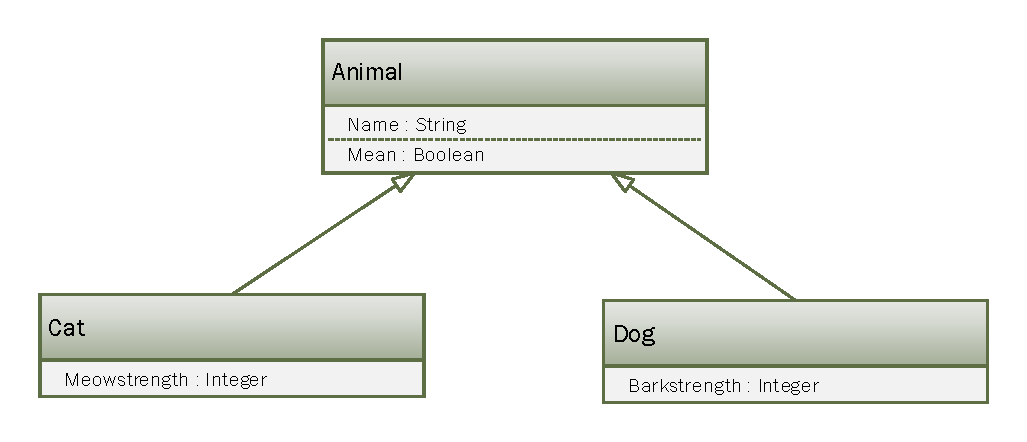
\includegraphics[width=\textwidth]{Images/Klassendiagramm.pdf}
    \caption{Klassendiagramm \\ in Anlehnung an \cite[]{WilliamKennedy.2013}}
    \label{fig:Klassendiagramm}
\end{figure}

\autoref{fig:Klassendiagramm} zeigt ein UML-Klassendiagramm mit einer einfachen Vererbungs-Hierarchie.
Die beiden Klassen \emph{Cat} und \emph{Dog} erben die Eigenschaften der Klasse \emph{Animal}.


Da Go keine Vererbung beherrscht, ist Komposition die einzige Möglichkeit eine Hierarchie abzubilden \cite[]{Kennedy.2016}.
Das \autoref{lst:VererbungGo} zeigt die Implementierung der Vererbungshierarchie aus \autoref{fig:Klassendiagramm}.

\begin{listing}[H]
\caption{Vererbung in Go \\ Quelle:\cite{Kennedy.2016}}
\label{lst:VererbungGo}
\begin{GoCode}
type Animal struct {
    Name string
    mean bool
}

type Cat struct {
    Basics Animal
    MeowStrength int
}

type Dog struct {
    Animal
    BarkStrength int
}
\end{GoCode}
\end{listing}

In Zeile 1-4 von \autoref{lst:VererbungGo} wird eine neue struct \emph{Animal} definiert.
Die struct \emph{Animal} wird anschließend in die structs \emph{Cat} und \emph{Dog} eingebunden. 
Hierdurch bekommen \emph{Cat} und \emph{Dog} die Eigenschaften von \emph{Animal}.
Bei der struct \emph{Cat} wurde die struct \emph{Animal} mit dem Zusatz \emph{Basics} eingebunden. 
Dies bedeutet, dass beim Zugriff auf die geerbten Eigenschaften aus \emph{Animal} zusätzlich \emph{Basics} angegeben werden muss. 
Die struct \emph{Dog} bindet \emph{Animal} dagegen anonym ein. 
Die anonyme Variante hat den Vorteil, dass beim Zugriff auf Eigenschaften nicht zwischen geerbten und eigenen Eigenschaften unterschieden werden muss.
Ist dieses Verhalten explizit gewünscht, sollte der Programmierer der eingebetteten struct einen Namen geben.
Da es sich bei diesem Vorgehen um eine Konvention handelt, sollte dieser Name immer gleich lauten und für größere Projekte separat festgehalten werden. 

Von Pike, einem der Entwickler von Go, wird der Verzicht auf Vererbung mit folgender Aussage begründet:
\begin{quote}
\enquote{Go takes an unusual approach to object-oriented programming, allowing methods on any type, not just classes, but without any form of type-based inheritance like subclassing. This means there is no type hierarchy. This was an intentional design choice. Although type hierarchies have been used to build much successful software, it is our opinion that the model has been overused and that it is worth taking a step back.}\cite[]{RobPike.2012}
\end{quote}

Swift kennt sowohl Strukturen als auch Klassen. Von Apple werden Klassen und Strukturen wie folgt beschrieben:
\begin{quote}
\enquote{Classes and structures are general-purpose, flexible constructs that become the building blocks of your program’s code. You define properties and methods to add functionality to your classes and
structures by using exactly the same syntax as for constants, variables, and functions.} \cite[S.183]{Apple.2017}
\end{quote}

Im Folgenden werden aus der Sicht von Swift nur Klassen berücksichtigt und Strukturen nicht beachtet.
\autoref{lst:VererbungSwift} zeigt die Implementierung der Vererbungshierarchie aus \autoref{fig:Klassendiagramm}.

\begin{listing}[H]
\caption{Vererbung in Swift}
\label{lst:VererbungSwift}
\begin{SwiftCode}
class Animal{
    var Name : String = ""
    var mean : Bool = false
}

class Cat : Animal{
    var MeowStrength : Int = 0
}

class Dog : Animal{
    var BarkStrength : Int = 0
}
\end{SwiftCode}
\end{listing}

In Zeile 1 - 4 wird die Basisklasse \emph{Animals} definiert. 
Die beiden Klassen \textit{Cat} und \textit{Dog} leiten sich von der Basisklasse \textit{Animal} ab. 
Dazu wird jeweils in Zeile 6 und Zeile 10 der Name der Basisklasse nach dem Namen der abgeleiteten Klasse getrennt von einem Doppelpunkt geschrieben \cite[S.226]{Apple.2017}.
Die abgeleiteten Klassen erben somit die Eigenschaften der Basisklasse. 

Im Gegensatz zu Go beherrscht Swift den Mechanismus der Vererbung.
Eine Klasse in Swift kann immer nur von genau einer Basisklasse abgeleitet werden, bekannt als einfache Vererbung \cite[S.125]{Hoffman.2017}.

\section{Datenkapselung}
Während die strukturierte Programmierung Daten und Logik voneinander trennt, gehören in der objektorientierten Programmierung die Daten explizit zu einem Objekt. 
Der direkte Zugriff auf die Daten eines Objekts ist nicht erlaubt. 
So haben Objekte das alleinige Recht lesend und schreibend auf ihre Daten zuzugreifen. 
Ein Zugriff auf die Daten von Außen muss über eine klar definierte Schnittstelle erfolgen.
In \autoref{fig:Kapselung} ist dargestellt, wie der direkte Zugriff auf die Daten unterbunden ist und nur durch die Methoden \emph{move} und \emph{paint} ermöglicht wird \cite[]{Lahres.2011}.

\begin{figure}[H]
    \centering
    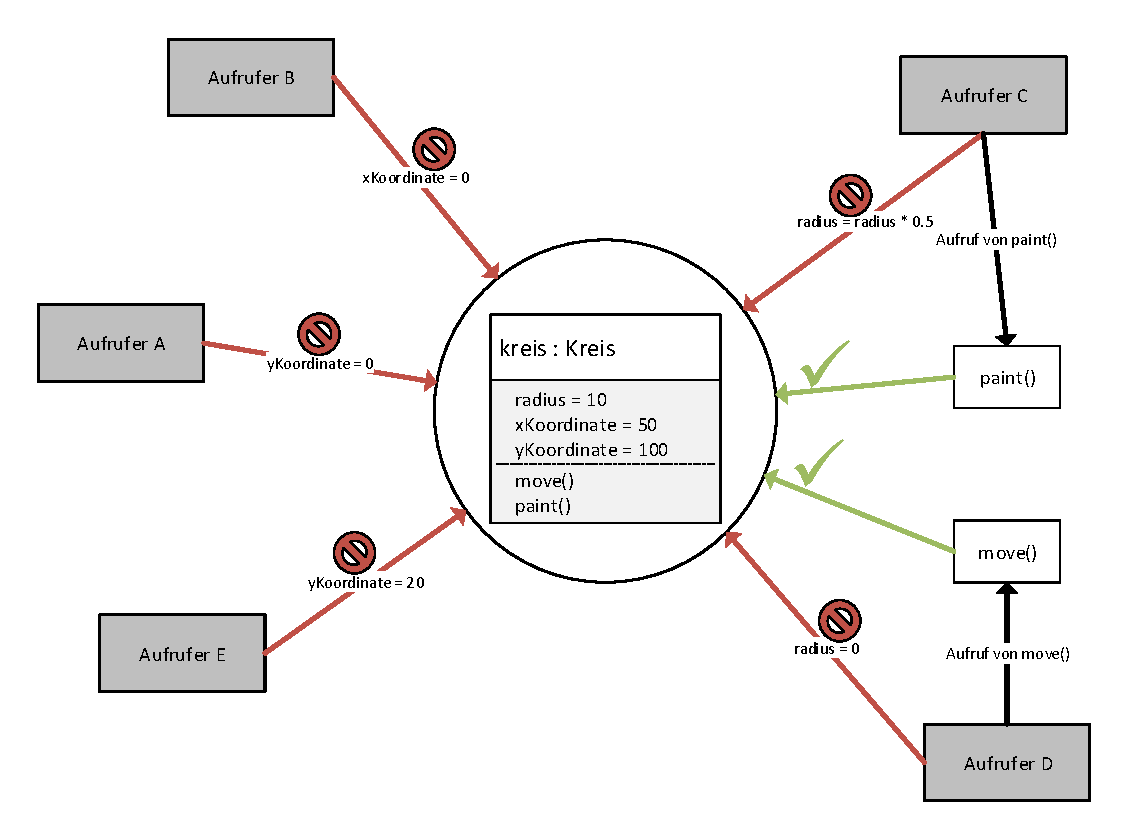
\includegraphics[height=8cm]{Images/Kapselung.pdf}
    \caption{Datenkapselung \\ in Anlehnung an \cite[]{Lahres.2011}}
    \label{fig:Kapselung}
\end{figure}

Ein Vorteil der Datenkapselung ist laut \cite[]{Lahres.2011}, dass ein Objekt selbst für die Konsistenz seiner Daten sorgen kann. 
Von \cite[S.86f]{PoetzschHeffter.2009} wird als Vorteil das Prinzip des \emph{Information Hiding} genannt. 
Da auf die Daten nur über eine definierte Schnittstelle zugegriffen werden kann, ist es möglich Implementierungsdetails hinter der Schnittstelle zu ändern ohne dass Programmteile, die diese Klasse verwenden, angepasst werden müssen. 
Dies setzt voraus, dass die Schnittstelle gleich bleibt.

Um den Zugriff auf die Daten eines Objektes zu unterbinden oder zu ermöglichen, bietet Go die Möglichkeit die Eigenschaften eines Objektes, ähnlich der Zugriffsmodifizierer in Java, entweder \emph{Public} oder \emph{Private} zu deklarieren. 
Im Unterschied zu Java verwendet Go allerdings keine Schlüsselwörter wie \emph{Public} oder \emph{Private}.
Wird in Go der erste Buchstabe des Names eines Typs, Variable/Konstante oder Funktion klein geschrieben, ist das Element nur innerhalb des \emph{Package} sichtbar, also Private. 
Wird der erste Buchstabe des Names jedoch groß geschrieben, ist das Element auch außerhalb des \emph{Package} sichtbar, also Public.
Das \autoref{lst:KapselungGo} zeigt ein Beispiel für diesen Mechanismus. 
In Zeile 6 wird eine Eigenschaft \emph{age} definiert, die aufgrund der Kleinschreibung nicht aus dem Package \emph{animals} exportiert wird. 

\begin{listing}[H]
\caption{Datenkapselung in Go \\ Quelle:\cite[]{Kennedy.GoExport}}
\label{lst:KapselungGo}
\begin{GoCode}
package animals

type Dog struct {
    Name string
    BarkStrength int
    age int
}
\end{GoCode}
\end{listing}

Eine Anwendung der struct \emph{Dog} ist in \autoref{lst:KapselungGo2} zu sehen.
Nachdem in Zeile 5 das Package \emph{animals} importiert wurde, kann die struct \emph{Dog} verwendet werden.
Da die Eigenschaft \emph{age} nicht aus dem Package \emph{animals} exportiert wird, gibt der Compiler die Fehlermeldung aus Zeile 17 aus. 

\begin{listing}[H]
\caption{Datenkapselung in Go \\ Quelle:\cite[]{Kennedy.GoExport}}
\label{lst:KapselungGo2}
\begin{GoCode}
package main

import (
    "fmt"
    "animals"
)

func main() {
    dog := animals.Dog{
        Name:         "Chole",
        BarkStrength: 10,
        age:          5,
    }
    fmt.Printf("Counter: %#v\n", dog)
}
//Compiler-Fehler: 
//./main.go:14: unknown animal.Dog field ‘age’ in struct literal
\end{GoCode}
\end{listing}

Eine Möglichkeit die Eigenschaft \emph{age} zugänglich zu machen, ist es, den Zugriff über eine Get-Funktion und Set-Funktion zu realisieren.
Hierzu wurde im \autoref{lst:KapselungGo3} jeweils eine Funktion für den lesenden und schreibenden Zugriff auf die Eigenschaft \emph{age} implementiert. 
Die beiden Funktionsnamen setzen sich aus dem Namen der jeweiligen Eigenschaft, hier \emph{Age} und einem Prefix, \emph{Get} oder \emph{Set}, zusammen.
Es ist zu beachten, dass die Namen der beiden Funktionen (\emph{SetAge} und \emph{GetAge}) mit einem Großbuchstaben beginnen, da diese sonst nicht exportiert werden. 
Um den Ansatz der Datenkapselung konsequent zu verfolgen, sollten im \autoref{lst:KapselungGo3} auch die Eigenschaften \emph{Name} und \emph{BarkStrength} auf diese Art implementiert werden.   

\begin{listing}[H]
\caption{Datenkapselung in Go}
\label{lst:KapselungGo3}
\begin{GoCode}
package animals

type Dog struct {
    Name string
    BarkStrength int
    age int
}

func (d *Dog) SetAge(age int) {
    d.age = age
}

func (d *Dog) GetAge() int {
    return d.age
}
\end{GoCode}
\end{listing}

Auch Swift bietet Möglichkeiten zur Zugriffskontrolle. 
Die Zugriffs-Level sind relativ zu der Quellcodedatei und dem Modul, in dem die Entität definiert wurde \cite[S.394]{Apple.2017}.
Laut der offiziellen Dokumentation \cite[S.394]{Apple.2017} bietet Swift die folgenden fünf Zugriffs-Level:

\begin{itemize}
    \item Open access
    \item Public access
    \item Internal access
    \item File-private access
    \item Private access
\end{itemize}

Eine Entität, die als \textit{open} oder \textit{public} deklariert wurde, kann aus jeder Quellcodedatei im gleichen Modul verwendet werden. 
Ebenso kann jede Quellcodedatei, welche das Modul importiert, in dem die Entität definiert wurde, auf die Entität zugreifen. 
Das Schlüsselwort \textit{open} greift nur bei Klassen und deren Eigenschaften.
Eine Klasse, die als \textit{open} deklariert wurde, kann auch außerhalb ihres eigenen Moduls vererbt werden, wenn das zugehörige Modul importiert wurde.
Dies unterscheidet das \textit{open}-Zugriffslevel von dem \textit{public}-Zugriffslevel.
Wird eine Entität als \textit{internal} definiert, ist diese lediglich in Quellcodedateien des eigenen Moduls verfügbar. 
Das Zugriffslevel \textit{fileprivate} schränkt den Zugriff auf die eigene Quellcodedatei ein.
Das restriktivste Zugriffslevel \textit{private} schränkt den Zugriff auf die umschließende Deklaration, beispielsweise eine Klasse, ein.
Ist kein Zugriffslevel definiert, verwendet der Compiler das \textit{internal}-Zugriffslevel.

\begin{listing}[H]
\caption{Zugriffslevel in Swift \\ Quelle:\cite[S.396]{Apple.2017}}
\label{lst:ZugriffslevelSwift}
\begin{SwiftCode}
public class SomePublicClass {}
internal class SomeInternalClass {}
fileprivate class SomeFilePrivateClass {}
private class SomePrivateClass {}

public var somePublicVariable = 0
internal let someInternalConstant = 0
fileprivate func someFilePrivateFunction() {}
private func somePrivateFunction() {}
\end{SwiftCode}
\end{listing}

Neben der Möglichkeit den Zugriff zu beschränken, bietet Swift die Möglichkeit Getter/Setter zu verwenden.
\autoref{lst:DatenkapselungSwfit} zeigt ein Beispiel für Datenkapselung in Swift. 
Das Beispiel wurde analog zu dem \autoref{lst:KapselungGo3} in Go implementiert.

\begin{listing}[H]
\caption{Datenkapselung in Swift}
\label{lst:DatenkapselungSwfit}
\begin{SwiftCode}
class Dog {
    var Name : String = ""
    var BarkStrength : Int = 0
	
    private var _age : Int = 0
    public var Age : Int {
        get{return _age}
        set{_age = newValue}
    }
}
\end{SwiftCode}
\end{listing}

Die verschiedenen Zugriffslevel in Swift ermöglichen es, den Zugriff auf Entitäten viel feiner zu steuern als in Go.
Die Möglichkeit von Go, Entitäten als \textit{private} zu deklarieren (Kleinschreibung des Namens), ist in Swift mit dem Zugriffslevel \textit{internal access} vergleichbar (Schlüsselwort \textit{internal}). 
Wird in Go eine Entität als \textit{public} deklariert (Großschreibung des Namens), ist dies mit dem Zugriffslevel \textit{public access} (Schlüsselwort \textit{public}) in Swift zu vergleichen.
Der Einsatz von Getter/Setter-Methoden in Swift ermöglicht dem Programmierer eine einfachere Schreibweise von Zuweisungen. 
In \autoref{lst:GetterSetterSWift} ist die Verwendung der Klasse aus \autoref{lst:DatenkapselungSwfit} zu sehen. 
Der Variablen \textit{aDog} wird eine neue Instanz der Klasse \textit{Dog} zugewiesen.
Anschließend wird der Instanzvariablen \textit{Age} der Wert 2 zugewiesen.

\begin{listing}[H]
\caption{Einsatz von Getter/Setter in Swift}
\label{lst:GetterSetterSWift}
\begin{SwiftCode}
var aDog = Dog()

aDog.Age = 2

\end{SwiftCode}
\end{listing}

In Go sieht die Verwendung von Getter/Setter-Methoden aus, wie in \autoref{lst:GetterSetterGo} abgebildet.
Da Go keine expliziten Getter/Setter-Methoden unterstützt, ist das Vorgehen aus \autoref{lst:KapselungGo3} und \autoref{lst:GetterSetterGo} an die Konvention gebunden, dass Instantzvariablen \textit{private} sind und der Zugriff auf die Werte der Instanzvariablen rein über eigens implementierte Getter/Setter-Methoden erfolgt.
Um das Konzept der Datenkapselung in Go zu verfolgen, muss diese Konvention eingehalten werden.
Swift erleichtert es dem Entwickler, dieses Konzept zu verfolgen.

\begin{listing}[H]
\caption{Einsatz von Getter/Setter in Go}
\label{lst:GetterSetterGo}
\begin{GoCode}
var Dog = new(animals.Dog)

Dog.SetAge(2)
\end{GoCode}
\end{listing}

\section{Polymorphie}
Neben Vererbung und Datenkapselung ist \textit{Polymorphie} ein Grundelement der objektorientierten Programmierung.
\cite[]{Lahres.2011} versteht unter \textit{Polymorphie} in der objektorientierten Programmierung, dass verschiedene Objekte bei Aufruf derselben Operation unterschiedliches Verhalten zeigen können. 
In \autoref{fig:Polymorphie} wird ein praktisches Beispiel für Polymorphie aus dem Alltag gezeigt. 

\begin{figure}[H]
    \centering
    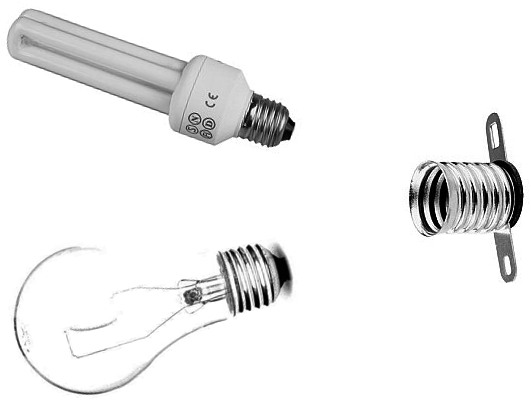
\includegraphics[height=5cm]{Images/Polymorphie}
    \caption{Beispiel für Polymorphie \\ Quelle:\cite[]{Lahres.2011}}
    \label{fig:Polymorphie}
\end{figure}

Polymorphie wird von \cite[]{Lahres.2011} mit ,,Vielgestaltigkeit'' übersetzt. Das Beispiel von \cite[]{Lahres.2011} bezieht sich auf die in \autoref{fig:Polymorphie} abgebildeten Glühbirnen und die zugehörige Fassung. 
Eine Glühbirne kann unterschiedliche Formen und Stärken haben, aber solange sie sich an die Norm für die Fassung hält, wird sie in der Fassung funktionieren. 
In Bezug auf Objektorientierung nennt \cite[]{Lahres.2011} das Beispiel ein Berechnungsverfahren gegen ein effizienteres Berechnungsverfahren zu tauschen. 
Hierzu muss nur das Berechnungsverfahren, die Glühbirne, gegen eine neue Implementierung getauscht werden und in die vorhergesehene ,,Fassung'' geschraubt werden.

\begin{quote}
\enquote{An den richtigen Punkten eingesetzt, kann die Nutzung der Polymorphie dadurch zu wesentlich flexibleren Programmen führen. Sie steigert damit die Wartbarkeit und Änderbarkeit unserer Software.}
\cite[]{Lahres.2011}
\end{quote}

An dieser Stelle soll der Einsatz von Polymorphie in Go und Swift untersucht werden. 
Nach Ansicht von \cite[]{WilliamKennedy.2013} ist Vererbung ohne Polymorphie nutzlos und die Art der Implementierung von Interfaces in Go macht Vererbung überflüssig. 
Als Grundlage dient das \autoref{lst:VererbungGo}. 

\begin{listing}[H]
\caption{Polymorphie in Go \\ in Anlehung an \cite[]{WilliamKennedy.2013}}
\label{lst:PolymorhpieGo}
\begin{GoCode}
package main

import (
    "fmt"
)

type Animal struct {
    Name string
    mean bool
}

type AnimalSounder interface {
    MakeNoise()
}

type Dog struct {
    Animal
    BarkStrength int
}

type Cat struct {
    Basics Animal
    MeowStrength int
}

func (animal *Animal) PerformNoise(strength int, sound string) {
    if animal.mean == true {
        strength = strength * 5
    }

    for voice := 0; voice < strength; voice++ {
        fmt.Printf("%s ", sound)
    }

    fmt.Println("")
}

func (dog *Dog) MakeNoise() {
    dog.PerformNoise(dog.BarkStrength, "BARK")
}

func (cat *Cat) MakeNoise() {
    cat.Basics.PerformNoise(cat.MeowStrength, "MEOW")
}

func MakeSomeNoise(animalSounder AnimalSounder) {
    animalSounder.MakeNoise()
}
\end{GoCode}
\end{listing}

Im Unterschied zu \autoref{lst:VererbungGo} wurde in \autoref{lst:PolymorhpieGo} den Objekten ein Verhalten in Form von Methoden gegeben.
Im Interface \emph{AnimalSounder} ist eine Funktion \emph{MakeNoise()} definiert. 
Dieses Interface wird von \emph{Dog} (Zeile 28 - 39) und \emph{Cat} (Zeile 42 - 44) implementiert. 
Sobald in Go ein Type ein Interface implementiert, repräsentiert dies das Interface. 
Die Implementierungen des Interfaces rufen wiederum die auf dem Type \emph{Animal} implementierte Funktion \emph{PerformNoise} auf.
Der Funktion \emph{MakeSomeNoise} wird ein Übergabeparameter vom Typ des Intefaces \emph{Animalsounder} übergeben. 
Das Interface \emph{AnimalSounder} und die Funktion \emph{MakeSomeNoise} sorgen für das polymorphe Verhalten \cite[]{WilliamKennedy.2013}.  

Das \autoref{lst:PolymorhpieGo2} zeigt die Verwendung der Typen \emph{Dog} und \emph{Cat}.
Dazu wird jeweils eine Instanz vom Type \emph{Dog} und vom Type \emph{Cat} erstellt. 
Anschließend wird die Funktion \emph{MakeSomeNoise} jeweils mit den erzeugten Instanzen von \emph{Cat} und \emph{Dog} aufgerufen. 
Dies ist möglich, da \emph{Cat} und \emph{Dog} das Interface \emph{AnimalSounder} implementieren. 

\begin{listing}[H]
\caption{Polymorphie in Go \\ in Anlehung an \cite[]{WilliamKennedy.2013}}
\label{lst:PolymorhpieGo2}
\begin{GoCode}
package main

func main() {
    myDog := &Dog{
        Animal{
            "Rover", // Name
            false,   // mean
        },
        2, // BarkStrength
    }

    myCat := &Cat{
        Basics: Animal{
            Name: "Julius",
            mean: true,
        },
        MeowStrength: 3,
    }

    MakeSomeNoise(myDog)
    MakeSomeNoise(myCat)
}
//Ausgabe:
//BARK BARK
//MEOW MEOW MEOW MEOW MEOW MEOW MEOW MEOW MEOW MEOW MEOW 
//MEOW MEOW MEOW MEOW
\end{GoCode}
\end{listing}

Um in Swift Polymorphie zu implementieren, werden \textit{protocols} eingesetzt.
\textit{Protocols} sind ähnlich zu \textit{Interfaces} aus anderen Programmiersprachen wie Java und Go.
Von Apple werden \textit{protocols} wie folgt definiert:

\begin{quote}
\enquote{A protocol defines a blueprint of methods, properties, and other requirements that suit a particular
task or piece of functionality. The protocol can then be adopted by a class, structure, or enumeration
to provide an actual implementation of those requirements. Any type that satisfies the requirements of
a protocol is said to conform to that protocol.} \cite[S.341]{Apple.2017}
\end{quote}

In \autoref{lst:PolymorphieSwift1} ist die Swift-Implementierung von \autoref{lst:PolymorhpieGo} abgebildet.
Ähnlich einer Klasse kann ein \textit{Protocol} in Swift Eigenschaften und Methoden haben. 
In Zeile 17 - 19 wird das Protocol \textit{AnimalSounder} definiert. 
Das Protocol \textit{AnimalSounder} hat nur eine Methode \textit{MakeNoise()}. 
Die Methode \textit{MakeNoise()} wird lediglich mit ihrer Signatur definiert. 
Es wird keine Methodenkörper definiert. 
Die Implementierung der Methode \textit{MakeNoise()} muss in den Klassen \textit{Dog} und \textit{Cat} geschehen.
In Zeile 1 - 15 wird die Basisklasse \textit{Animal} definiert. 
Die Methode \textit{PerformNoise} erwartet die beiden Übergabeparameter \textit{strength} und \textit{sound}.
Die Klassen \textit{Dog} und \textit{Cat} erben von der Basisklasse \textit{Animal}.
Bei der Implementierung der Methode \textit{MakeNoise} in den Klassen \textit{Dog} und \textit{Cat} wird die von der Klasse \textit{Animal} geerbte Methode \textit{PerformNoise} mit den spezifischen Parametern aufgerufen.

\begin{listing}[H]
\caption{Polymorphie in Swift I}
\label{lst:PolymorphieSwift1}
\begin{SwiftCode}
class Animal{
    var Name : String = ""
    var mean : Bool = false
	
    func PerformNoise(strength: Int, sound: String){
        var newStrength = strength
        if mean == true{
            newStrength = strength * 5
        }
		
        for _ in 0...newStrength{
            print(sound)
        }
    }
}

protocol AnimalSounder{
    func MakeNoise()
}

class Dog : Animal, AnimalSounder{
    var BarkStrength : Int = 0
	
    func MakeNoise() {
        PerformNoise(strength: BarkStrength, sound: "BARK")
    }
}

class Cat : Animal, AnimalSounder{
    var MeowStrength : Int = 0
	
    func MakeNoise() {
        PerformNoise(strength: MeowStrength, sound: "MEOW")
    }
}
\end{SwiftCode}
\end{listing}

\autoref{lst:PolymorphieSwift2} zeigt die Verwendung der Klassen aus \autoref{lst:PolymorphieSwift1}.
Die beiden Objekte \textit{myDog} und \textit{myCat} werden mit den gleichen Werten initialisiert, welche auch in der Implementierung in Go in \autoref{lst:PolymorhpieGo2} verwendet werden.
In Zeile 11 und 12 wird bei beiden Objekten die Methode \textit{MakeNoise} aufgerufen, welche zu der Ausgabe in Zeile 15 - 17 führt. 

\begin{listing}[H]
\caption{Polymorphie in Swift II}
\label{lst:PolymorphieSwift2}
\begin{SwiftCode}
var myDog = Dog()
myDog.Name = "Rover"
myDog.mean = false
myDog.BarkStrength = 2

var myCat = Cat()
myCat.Name = "Julius"
myCat.mean = true
myCat.MeowStrength = 3

myDog.MakeNoise()
myCat.MakeNoise()

//Ausgabe: 
//BARK BARK 
//MEOW MEOW MEOW MEOW MEOW MEOW MEOW MEOW MEOW MEOW MEOW 
//MEOW MEOW MEOW MEOW 
\end{SwiftCode}
\end{listing}

Es kann sowohl in Go als auch in Swift objektorientiert programmiert werden. 
Allerdings ist Go keine vollwertige objektorientierte Programmiersprache. 

\begin{quote}
\enquote{I consider Go to be a light object oriented programming language. Yes it does have encapsulation and type member functions but it lacks inheritance and therefore traditional polymorphism.} \cite[]{WilliamKennedy.2013}
\end{quote}

Swift hingegen kann als vollwertige objektorientierte Programmiersprache angesehen werden.

\begin{quote}
\enquote{Swift’s features allow it to be used as an object-oriented programming language. This
means that you do the majority of your work by creating and manipulating objects—
chunks of data and code that represent a thing that can perform some useful work or
store some useful data.} \cite[59]{Manning.2016}
\end{quote}

In den Codebeispielen konnten alle Anforderungen erfüllt werden.
Es muss jedoch berücksichtigt werden, dass es sich hierbei um einfache Anforderungen handelt, die nicht der Realität entsprechen. 
Das Go keine Vererbung unterstützt, ist im Vergleich zu Swift der größte Nachteil.
Die Art in der Objektorientierung in Swift umgesetzt ist, ist für Umsteiger von anderen objektorientierten Programmiersprachen (Java, C\#) einfacher zu erlernen und zu verstehen.
\cite[]{WilliamKennedy.2013} beschreibt die objektorientierten Fähigkeiten von Go wie folgt.

\begin{quote}
\enquote{Go took the best parts of OOP, left out the rest and gave us a better way to write polymorphic code.} \cite[]{WilliamKennedy.2013}
\end{quote}

\section{Erweiterungen}
Mit \textit{Xtend}\cite[]{Xtend} ist eine Programmiersprache für die \textit{Java Virtual Machine} verfügbar, welche es erlaubt über \textit{Extension Methods} neue Methoden zu bestehenden Klassen hinzuzufügen, ohne diese zu verändern.

Swift kennt diese Funktionalität unter dem Namen \textit{Extensions}.
Ein Auszug aus der Swift Dokumentation \cite[S331]{Apple.2017} bietet einen Überblick über die Möglichkeiten, die Extensions in Swift bieten:

\begin{itemize}
    \item \enquote{Add computed instance properties and computed type properties}    
    \item \enquote{Define instance methods and type methods}
    \item \enquote{Provide new initializers}
    \item \enquote{Define subscripts}
    \item \enquote{Define and use new nested types}
    \item \enquote{Make an existing type conform to a protocol}
\end{itemize}

\autoref{lst:SwiftExtensions} zeigt die Anwendung von \textit{Extensions} in Swift.
Der Swift-Basisdatentyp \textit{Double} wird über die \textit{Extension} mit \textit{Properties} für Längenangaben erweitert.
Eine \textit{Extension} kann bestehende Funktionalitäten eines Objektes nicht überschreiben.
Auch \textit{Protocols} können mit \textit{Extensions} erweitert werden.

\begin{listing}
\caption{\textit{Extensions} in Swift \\ Quelle:\cite[S.332f]{Apple.2017}}
\label{lst:SwiftExtensions}
\begin{SwiftCode}
extension Double {
    var km: Double { return self * 1_000.0 }
    var m: Double { return self }
    var cm: Double { return self / 100.0 }
    var mm: Double { return self / 1_000.0 }
    var ft: Double { return self / 3.28084 }
}

let oneInch = 25.4.mm
print("One inch is \(oneInch) meters") 
// Prints "One inch is 0.0254 meters"

let threeFeet = 3.ft
print("Three feet is \(threeFeet) meters")
// Prints "Three feet is 0.914399970739201 meters"
\end{SwiftCode}
\end{listing}

Go bietet dem Programmierer keine Möglichkeit bestehende Typen durch integrierte Sprachkonstrukte zu erweitern. 

\chapter{Fehlerbehandlung}

\section{Möglichkeiten zur Fehlerbehandlung}

\section{Exceptions}

\chapter{Tools}
Dieses Kapitel beschäftigt sich damit, wie eine Entwicklungsumgebung in Go und Swift aussehen könnte. 
% Welche Betriebssysteme werden unterstützt?
% Gibt es \gls{IDE} %integrierte Entwicklungsumgebungen?
% Welchen Umfang hat die Standardbibliothek?


\section{Entwicklungsumgebung}
Auf Github \cite[]{Github.Swift} werden für Swift die in \autoref{tab:UnterstützteBetriebssysteme} aufgeführten \textit{host development operationg systems} genannt.
In Go kann auf den in \autoref{tab:UnterstützteBetriebssysteme} gezeigten Plattformen entwickelt werden.

\begin{table}[H]
    \centering
    \begin{tabularx}{\textwidth}{ |X|X|X|X| }
    \hline 
    \rowcolor[gray]{0.75} \cellcolor{white} & \textbf{Windows} & \textbf{Linux} & \textbf{MacOS} \\
    \hline
    \cellcolor{Gray} \textbf{Go} Version 1.8.1 & Ab Windows XP & Ab Linux 2.6.23 & Ab MacOS X 10.8 \\
    \hline
    \cellcolor{Gray} \textbf{Swift} Version 3.1.1 &  & Ubuntu LTS und die letzte Ubuntu Version (Aktuell 16.10) & Xcode 8.3.2 \\
    \hline
    \end{tabularx}
    \caption{Unterstützte Betriebssysteme}
    \label{tab:UnterstützteBetriebssysteme}
\end{table}

Von \cite[]{TechnoPedia} wird eine Entwicklungsumgebung folgenderweise definiert.

\begin{quote}
\enquote{In software development, the development environment is a set of processes and tools that are used to develop a source code or program.}\cite[]{TechnoPedia}
\end{quote}

Eine einfache Entwicklungsumgebung besteht aus einem geeigneten Quelltext-Editor, Debugger und Compiler. Von \cite[]{NotUseIde} wird empfohlen, auf eine integrierte Entwicklungsumgebung (siehe \autoref{sec:IDE}) zu verzichten, um die hohe Lernkurve von \gls{IDE}s zu vermeiden.
Aus diesem Grund wurden alle Codebeispiele in dieser Arbeit mit einem Quelltext-Editor und den sprachspezifischen Werkzeugen entwickelt.
Als Quelltext-Editor wurde \textit{Visual Studio Code} eingesetzt. 
\textit{Visual Studio Code} zeichnet sich durch folgende Fähigkeiten aus:

\begin{itemize}
    \item Open Source
    \item Verfügbar für Windows, Linux und MacOS
    \item Durch \textit{Extensions} erweiterbar
    \item \textit{Extensions} für Go und Swift sind verfügbar
\end{itemize}

Die Installation von Swift und Go sowie Visual Studio Code wird hier nicht näher erläutert, da sich die Vorgehensweise von Version zu Version ändern kann.
Im Folgenden wird die Einrichtung einer Arbeitsumgebung, im weiteren Verlauf auch \textit{Workspace} genannt, für Go und Swift erläutert.

Die offizielle Dokumention von Go \cite[]{GoDoc.Workspaces} äußert sich folgenderweise zum allgemeinen Aufbau einer Arbeitsumgebung für Go:

\begin{itemize}
    \item \enquote{Go programmers typically keep all their Go code in a single workspace.}
    \item \enquote{A workspace contains many version control repositories (managed by Git, for example).} 
    \item \enquote{Each repository contains one or more packages.}
    \item \enquote{Each package consists of one or more Go source files in a single directory.}
    \item \enquote{The path to a package's directory determines its import path.}
\end{itemize}

Der grundsätzliche Aufbau einer Arbeitsumgebung in Go ist in \autoref{fig:GoWorkspace} zu sehen. 

\begin{figure}[H]
    \centering
    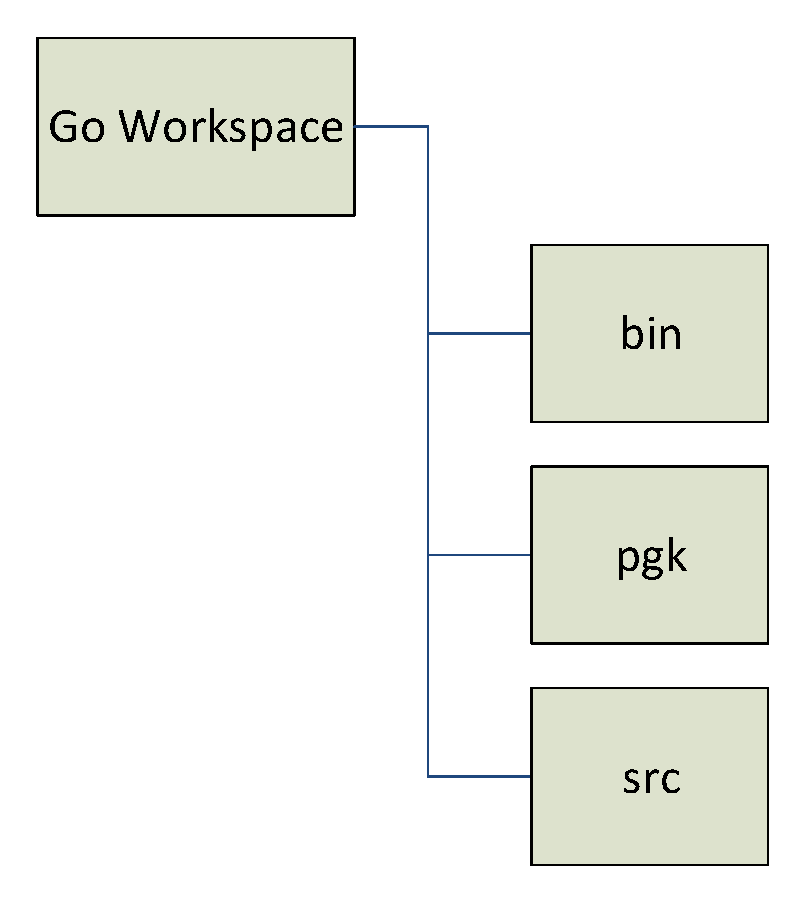
\includegraphics[height=6cm]{Images/GoWorkspace}
    \caption{Aufbau einer Arbeitsumgebung in Go}
    \label{fig:GoWorkspace}
\end{figure}

Wird Quelltext kompiliert, werden die vom Compiler erzeugten Binärdateien in den Ordner \textit{bin}, für ausführbare Progamme, und \textit{pkg}, für eigene Bibliotheken, abgelegt.

Im Ordner \textit{src} befindet sich der Quelltext, üblicherweise in Form von Repositorys eines Versionskontrollsystems.

Swift unterscheidet sich hier von Go. 
In Swift gibt es einzelne Arbeitsbereiche für jedes Projekt. 
Zudem ist es möglich, sich diese Arbeitsbereiche mit dem Tool \textit{Swift Package Manager}, welches bei der Installation von Swift mitgeliefert wird, Arbeitsbereiche automatisiert anlegen zu lassen.

\begin{listing}[H]
\caption{Anwendung des \textit{Swift Package Managers} \\ Quelle:\cite[S.22]{Hoffman.2017}}
\label{lst:SwiftPackageManager}
\begin{Commandline}
mkdir PMExample

cd PMExample

swift package init
\end{Commandline}
\end{listing}

\autoref{fig:SwiftWorkspace} zeigt den Aufbau des Arbeitsbereichs, nach Ausführen des \textit{Swift Package Managers} mit dem Befehl \textit{init}. 

\begin{figure}[H]
    \centering
    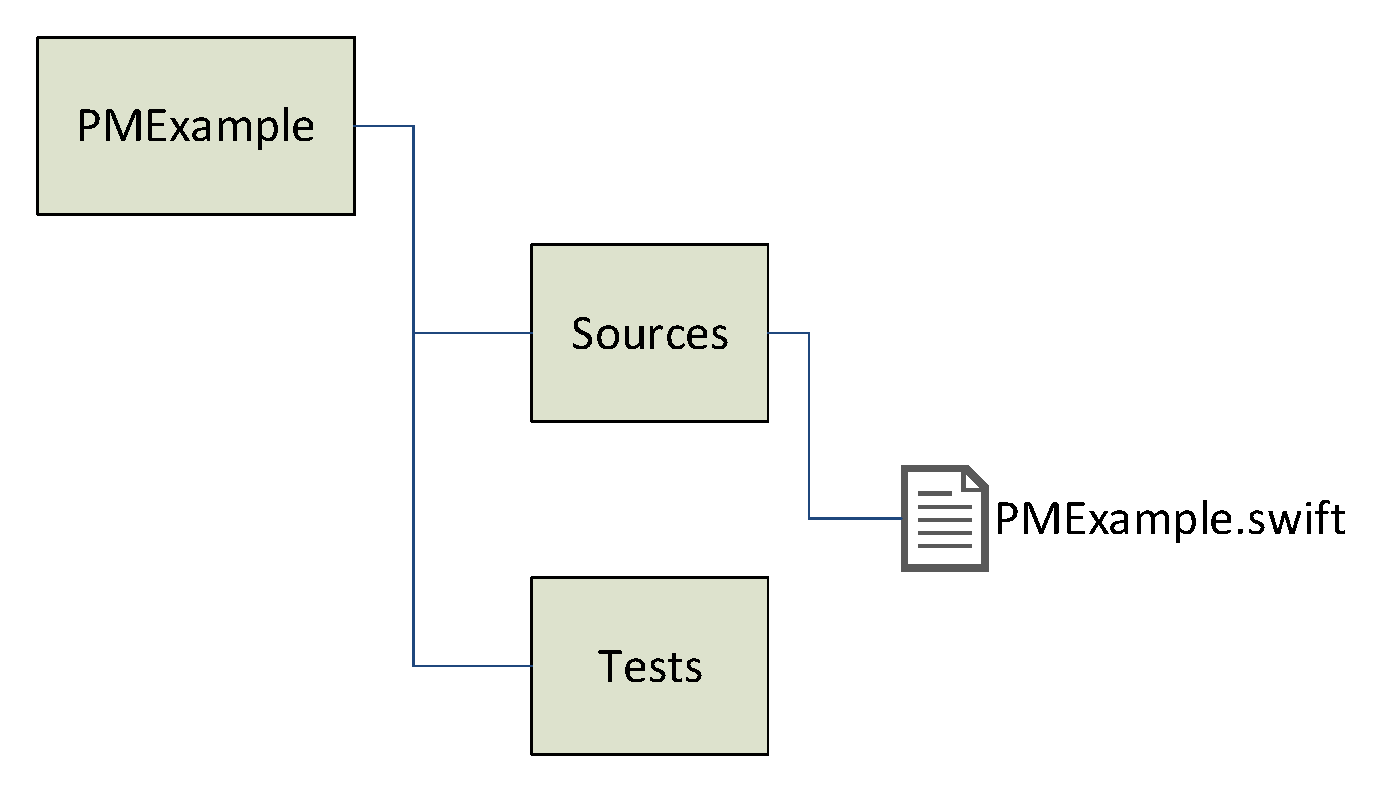
\includegraphics[height=6cm]{Images/SwiftWorkspace}
    \caption{Ein mit dem Swift Package Manager angelegter Workspace}
    \label{fig:SwiftWorkspace}
\end{figure}

Der \textit{Swift Package Manager} legt, in dem in \autoref{lst:SwiftPackageManager} angelegten Verzeichnis, die Verzeichnisse \textit{Sources} u. \textit{Tests} an.
Zusätzlich wird die Datei \textit{PMExample.swift} im Verzeichnis \textit{Sources} angelegt.

\section{Integrierte Entwicklungsumgebungen}
\label{sec:IDE}
Dieser Abschnitt soll einen Marktüberblick über die für Swift und Go vefügbaren integrierten Entwicklungsumgebungen bieten.
Eine integrierte Entwicklungsumgebung vereint laut \cite[]{TechnoPedia} die folgenden Fähigkeiten:

\begin{itemize}
    \item Editieren von Quelltext
    \item Build-Prozess ausführen
    \item Tests ausführen
    \item Debugging
\end{itemize}

Derzeit gibt es mit \textit{LiteIDE} (https://github.com/visualfc/liteide) nur eine richtige integrierte Entwicklungsumgebung für Go.
\textit{LiteIDE} ist auf folgenden Plattformen verfügbar als Open-Source verfügbar:

\begin{itemize}
    \item Windows 
    \item Linux
    \item MacOS X ab Version 10.6
    \item FreeBSD ab Version 9.2
    \item OpenBSD ab Version 5.6
\end{itemize}

Die Firma Jetbrains hat angekündigt mit \textit{Gogland}\cite[]{Gogland} eine integrierte Entwicklungsumgebung für Swift auf den Markt zu bringen, siehe \cite[]{Gogland.Heise}.
\textit{Gogland} befindet sich allerdings derzeit noch im \textit{Early Access Program}, einer Vorabversion.

Swift ist zwar für Linux und MacOS verfügbar, jedoch gibt es mit XCode nur eine integrierte Entwicklungsumgebung für MacOS.

\section{Standardbibliothek}
Apple beschreibt die Standardbibliothek von Swift mit folgendem Satz.
\begin{quote}
\enquote{The Swift language is relatively small, because many common types, functions, and operators that appear virtually everywhere in Swift code are actually defined in the Swift standard library.} \cite[S.427]{Apple.2017}
\end{quote}

Von \cite[S.184]{Kennedy.2016} wird ein Vorteil bei Verwendung der Go Standardbibliothek genannt. 

\begin{quote}
\enquote{By using packages from the standard library, you make it easier to manage your code and ensure that it’s reliable. This is because you
don’t have to worry if your program is going to break between release cycles, nor do
you have to manage third-party dependencies.} \cite[S.185]{Kennedy.2016}
\end{quote}

Die Standardbibliothek, sowohl von Go als auch Swift, ist also ein wichtiger Bestandteil der Programmiersprache. 
Laut \cite[S.185]{Kennedy.2016} beinhaltet die Standardbibliothek von Go über 100 Packages, welche in 38 Kategorien unterteilt sind.

Mit der dritten Version von Swift gelang es den Entwicklern, den Quellcode von Swift \textit{source-compatible} zu machen.
Dies bedeutet, dass der Quellcode von Swift auf allen unterstützen Plattformen (siehe \autoref{tab:UnterstützteBetriebssysteme}) kompiliert werden kann \cite[S.8]{Hoffman.2017}.
Eine ausführliche Standardbibliothek ist wichtig und minimiert die Abhängigkeit von externen Bibliotheken.





\chapter{Speicherverwaltung}
Speicherverwaltung hat einen großen Einfluss darauf, wie eine Programmiersprache in der Praxis arbeitet. 
Besonders in C{\textbackslash}C++ muss der Entwickler viel Aufwand in das Reservieren und Freigeben von Speicher investieren.
Die heutigen Anforderung an eine nebenläufige objektorientierte Programmiersprache erfordern eine automatische Speicherverwaltung, da der Besitz eines Speicherfragments bei nebenläufigen Ausführungen nur schwer manuell zu verwalten ist \cite{RobPike.2012}.

\section{Garbage Collection}
Go verwendet zur Speicherverwaltung einen \textit{Garbage Collector}. 
% Eine Meinung, die unter Entwicklern vertreten wird ist, dass \textit{Garbage Collection} Leistung kostet. 
Einige Programmierer sind der Ansicht, dass \textit{Garbage Collection} Leistung kostet.
Die FAQ von Google liefert auf die Fragestellung, warum Go mit \textit{Garbage Collection} arbeitet, folgende Antwort.

\begin{quote}
\enquote{We feel it's critical to eliminate that programmer overhead, and advances in garbage collection technology in the last few years give us confidence that we can implement it with low enough overhead and no significant latency.}\cite{Golang.FAQ}
\end{quote}

Go bietet dem Entwickler keine Möglichkeit explizit Speicher freizugeben, nur der \textit{Garbage Collector} kann Speicher freigeben \cite{RobPike.2012}.
Der \textit{Garbage Collector} von Go ist als \textit{tri-color}, \textit{mark-sweep Collector} implementiert.
Auf dem offiziellen Go Blog wir die Funktionsweise folgendermaßen beschrieben:

\begin{quote}
\enquote{In a tri-color collector, every object is either white, grey, or black and we view the heap as a graph of connected objects. At the start of a GC cycle all objects are white. The GC visits all roots, which are objects directly accessible by the application such as globals and things on the stack, and colors these grey. The GC then chooses a grey object, blackens it, and then scans it for pointers to other objects. When this scan finds a pointer to a white object, it turns that object grey. This process repeats until there are no more grey objects. At this point, white objects are known to be unreachable and can be reused.} \cite{Go.GC}
\end{quote}

Swift verwendet als \textit{Garbage Collector} \textit{Automatic Reference Counting}(ARC).
\textit{Automatic Reference Counting} merkt sich die Referenzen auf Instanzen von Klassen.
Zeigt keine Referenz auf die Instanz einer Klasse, wird diese Instanz von \textit{Automatic Reference Counting} zerstört und der Speicher frei gegeben \cite[S.137]{Hoffman.2017}. 
Dieses Verhalten von \textit{Automatic Reference Counting} funktioniert in den meisten Fällen.
In seltenen Fällen muss der Entwickler seinen Quelltext anpassen um das Verhalten von \textit{Automatic Reference Counting} zu verbessern.

Wie bereits zu Anfang dieses Kapitels erwähnt, ist Speicherverwaltung besonders hinsichtlich nebenläufiger Programmierung ein wichtiger Punkt.
Go und Swift nehmen dem Programmierer durch ihre Mechanismen zur Speicherverwaltung einen Großteil der Arbeit ab. 
Ein manuelles Eingreifen in die Speicherverwaltung ist nur dann nötig, wenn im Besonderen auf Leistung geachtet werden muss oder der Programmierer gezielt die Speicherverwaltung beinflussen möchte.



\input{Hauptteil/Nebenläufigkeit.tex}

\chapter{Funktionale Programmierung}
Um zu analysieren, inwieweit Swift und Go funktionale Programmierung ermögliche, muss zunächst erläutert werden, was unter funktionaler Programmierung zu verstehen ist.
Piepmeyer beantwortet in \cite[S.6]{Piepmeyer.2010} die Frage ,,Wann ist eine Sprache Funktional'' folgendermaßen:

\begin{itemize}
    \item In funktionalen Sprachen können Funktionen anonym definiert werden
    \item Funktionen werden wie alle anderen Daten behandelt
\end{itemize}

Von Esser werden in \cite[S.243]{Esser.2011} zwei Begriffe genannt, welche funktionale Programmiersprachen erfüllen und bei prozeduralen Programmiersprachen fehlen.

\begin{itemize}
    \item First-Class Function
    \item High-Order Function
\end{itemize}

Von Piepmeyer wird ein erheblicher Vorteil der funktionalen Programmierung genannt.

\begin{quote}
\enquote{In der funktionalen Programmierung hängt das Ergebnis einer Berechnung nicht vom Zeitpunkt der Berechnung ab. Aufgrund dieser referentiellen Transparenz können funktionale Programme leicht parallelisiert werden.} \cite[S.13]{Piepmeyer.2010}
\end{quote}

% Dieses Kapitel soll zeigen, ob mit Go und Swift funktional programmiert werden kann.
Nachfolgend soll erläutert werden, ob mit Go und Swift funktional programmiert werden kann.

\section{Anonyme Funktionen}
Ein Merkmal von funktionalen Programmiersprachen ist die Möglichkeit eine Funktion anonym, also ohne Namen, zu definieren \cite[S.28]{Piepmeyer.2010}.
% Anonyme Funktionen sind auch als \textit{Closures} beziehungsweise \textit{Lambda Expressions} bekannt.
\cite[S.219]{Hoffman.2017} sieht anonyme Funktionen als Datentyp, der anstatt beispielsweise ganzzahligen Werten, einen Block Quellcode beinhaltet.

\begin{listing}[H]
\caption{Anonyme Funktion in Swift \\ Quelle:\cite[S.220]{Hoffman.2017}}
\label{lst:SwiftClosure}
\begin{SwiftCode}
let clos1 = {
    () -> Void in
    print("Hello World")
}
\end{SwiftCode}
\end{listing}

Ein Beispiel für eine anonyme Funktion in Go ist in \autoref{lst:GoFirstClassFunctions} in Zeile 15 - 17 zu sehen.

\section{First-Class Functions}
Um ein Gefühl für den Begriff \textit{First-Class Function} zu bekommen, leitet \cite[S.243f]{Esser.2011} das Thema mit einer Definition des Begriff \textit{First-Class Objects} aus der Objektorientierung ein.
Objekte werden als Werte gesehen, die über Referenzen, Parameter oder als Ergebnis weitergereicht werden.
Die Methoden eines Objekts sind nicht eigenständig, sondern können nur indirekt über das Objekt weitergegeben werden.
Der Begriff \textit{First-Class Function} dreht diese Sichtweise um.
Funktionen sind Werte, die über Referenzen, Parameter oder als Ergebnis an andere Funktionen weitergegeben werden.
Funktionen sind eigenständig und nicht an Objekte gebunden. 

\autoref{lst:GoFirstClassFunctions} zeigt die Anwendung von \textit{First-Class Functions} in Go.

\begin{listing}[H]
\caption{\textit{First-Class Functions} in Go \\ Quelle:\cite[]{Go.FirstClassFunctions}}
\label{lst:GoFirstClassFunctions}
\begin{GoCode}
package main

import "fmt"

func CallWith(f func(string), who string) {
    f(who)
}

type FunctionHolder struct {
    Function func(string)
}

func main() {
    holder :=   FunctionHolder{ 
                    func(who string) {
                        fmt.Println("Hello,", who) 
                    }
                }
                
    CallWith(holder.Function,"ernest")
}
\end{GoCode}
\end{listing}

In Zeile 5 - 7 wird eine Funktion \textit{CallWith} definiert, welche als Parameter eine Funktion und einen String übernimmt und anschließend die übergebene Funktion mit dem übergebenen String aufruft.
In Zeile 9 - 1 wird eine neuer Typ \textit{FunctionHolder} definiert, welcher eine Funktion mit einem String als Parameter aufnimmt.
In der \textit{main}-Funktion (Ab Zeile 13) wird zuerst eine neue Instanz des Typs \textit{FunctionHolder} erstellt und dieser mit einer anonymen Funktion, welche einen String entgegen nimmt, initialisiert.
Anschließend wird die Funktion \textit{CallWith} mit der in \textit{holder} gespeicherten Funktion und dem Literal ,,ernest'' aufgerufen.
Als Ergebnis wird ,,Hello, ernest'' ausgegeben. 

\section{High-Order Functions}
\textit{High-Order Functions} sind Funktionen, die eine Funktion als Übergabeparameter haben oder eine Funktion als Ergebnis liefern \cite[S.63]{Piepmeyer.2010}.

Im \autoref{lst:GoHighOrderFunctions} ist ein Beispiel für \textit{High-Order Functions} in Go zu sehen. 
In Zeile 11 wird ein neuer Type Namens \textit{strategy} definiert. 
Der Datentyp von \textit{strategy} ist eine Funktion.
Der Rückgabewert von \textit{strategy} ist vom Typ \textit{action} (Zeile 8), welcher wiederum eine Funktion darstellt.

\begin{listing}[H]
\caption{\textit{High-Order Functions} in Go \\ Quelle:\cite[]{Go.HighOrderFunctions}}
\label{lst:GoHighOrderFunctions}
\begin{GoCode}
// A score includes scores accumulated in previous turns for each player,
// as well as the points scored by the current player in this turn.
type score struct {
    player, opponent, thisTurn int
}

// An action transitions stochastically to a resulting score.
type action func(current score) (result score, turnIsOver bool)

// A strategy chooses an action for any given score.
type strategy func(score) action
\end{GoCode}
\end{listing}

\autoref{lst:SwiftHighOrderFunctions} zeigt ein Beispiel für \textit{High-Order Functions} in Swift.
Die Funktion \textit{aHigherOrderFunction} übernimmt als Parameter eine anonyme Funktion mit dem Name \textit{closure}.
In Zeile 5 - 7 wird eine anonyme Funktion definiert und der Konstante \textit{myClosure} zugewiesen.
In Zeile 9 wird \textit{myClosure} der Funktion \textit{aHigherOrderFunction} übergeben.

\begin{listing}[H]
\caption{\textit{High-Order Functions} in Swift \\ Quelle:\cite[]{Swift.HighOrderFunctions}}
\label{lst:SwiftHighOrderFunctions}
\begin{SwiftCode}
func aHigherOrderFunction(closure: () -> Void) {
    closure()
}

let myClosure = {
    print("Hello!")
}

aHigherOrderFunction(myClosure) // prints: Hello
\end{SwiftCode}
\end{listing}



% \section{Referentielle Transparenz}
% Als \textit{referentielle Transparenz} bezeichnet man die Eigenschaft einer Funktion, nur von den Werten seiner Teilfunktionen abhängig zu sein und nicht vom Zeitpunkt der Berechnung \cite[S.11]{Piepmeyer.2010}.




\chapter{Generische Programmierung}
Generische Programmierung erlaubt es flexible und wiederverwendbare Funktionen zu schreiben. 
Sie ermöglicht es Duplikation zu vermeiden und verständlichen Quelltext zu entwickeln \cite[S.371]{Apple.2017}.


Der FAQ von Go ist zu entnehmen, das Go derzeit keine generische Programmierung unterstützt. 
Jedoch ist es möglich, das Mechanismen zur generischen Programmierung im Laufe der Zeit in Go integriert werden \cite{Golang.FAQ}.


Swift bietet direkte Untestützung für generische Programmierung.
Laut \cite[S.371]{Apple.2017} sind Generics eine der mächtigsten Funktionen von Swift und weden auch in der Standardbibliothek von Swift ausgiebig genutzt.
Programmierer welche beispielweise aus dem Java-Umfeld kommen, sollten laut \cite[S.206]{Hoffman.2017} keine Probleme haben sich mit generischer Programmierung in Swift zurecht zu finden.
\autoref{lst:GenericFunctionSwift} zeit ein Beispiel für eine generische Funktion und \autoref{lst:GenericTypeSwift} ein Beispiel für eine generische Klasse.

\begin{listing}
\caption{Generische Funktion in Swift Quelle: \cite[S.373]{Apple.2017}}
\label{lst:GenericFunctionSwift}
\begin{SwiftCode}
func swapTwoValues<T>(_ a: inout T, _ b: inout T) {
    let temporaryA = a
    a = b
    b = temporaryA
}
\end{SwiftCode}
\end{listing}

\begin{listing}
\caption{Generische Klasse in Swift Quelle: \cite[S.213]{Hoffman.2017}}
\label{lst:GenericTypeSwift}
\begin{SwiftCode}
class List<T> {
    var items = [T]()
    
    func add(item: T) {
        items.append(item)
    }
    
    func getItemAtIndex(index: Int) -> T? {
        if items.count > index {
            return items[index]
        } else {
            return nil
        }
    }
}
\end{SwiftCode}
\end{listing}


\chapter{Anwendungsbeispiel}
Dieses Kapitel beschäftigt sich damit, die Machbarkeit der Implementierung eines konkreten Anwendungsbeispiels zu überprüfen.
Als Anwendungsbeispiel soll ein ,,Hallo Welt''-Beispiel in Form einer einfachen Webanwendung umgesetzt werden.
Zur Umsetzung soll ein Web-Framework eingesetzt werden.

% Dazu soll zuerst ein Überblick über die verfügbaren Frameworks gegeben werden und anschließend die beispielhafte Implementierung eines ,,Hallo Welt''-Beispiels in einem ausgewählten Framework für Go und Swift vorgestellt werden.

% \section{Frameworks}
% Die beiden Aufstellungen von Web-Frameworks für Go und Swift stellen lediglich einen Auszug aus den vorhandenen Frameworks dar.
% Das Augenmerk 

% Go:
% \begin{itemize}
%     \item Revel \cite{Revel} - 8326
%     \item Beego \cite{Beego} - 11105
%     \item Gin Gonic \cite{GinGonic} 10190
%     \item Iris \cite{Iris} 6946
%     \item Echo \cite{Echo} 7507
% \end{itemize}

% Swift:
% \begin{itemize}
%     \item Kitura \cite{Kitura} 5727
%     \item Perfect \cite{Perfect} 11601
%     \item Vapor \cite{Vapor} 9799
%     \item Express \cite{Express} 8534
% \end{itemize}

Zur Implementierung wurde für Go das Framework \textit{Beego}\cite{Beego} ausgewählt.
Das Framework \textit{Beego} wurde ausgewählt, da es auf Github die meisten Follower hat.
Um mit \textit{Beego} zu arbeiten, müssen die Quelltext-Dateien des Framworks in den eigenen \textit{Go-Workspace} heruntergeladen werden.
\autoref{lst:BeegoInstallation} zeigt in Zeile 1 den Befehl zur Installation von \textit{Beego}.

\begin{listing}[H]
\caption{Installation von \textit{Beego} Quelle:\cite{Beego}}
\label{lst:BeegoInstallation}
\begin{Commandline}
go get -u github.com/astaxie/beego
\end{Commandline}
\end{listing}

In Zeile 3 von \autoref{lst:BeegoInstallation} wird im Go-Workspace ein neuer Ordner angelegt und in diesen Ordner gewechselt.
\autoref{lst:HelloBeego} zeigt die die Datei \textit{hello.go}. 
Es wird ein neuer \textit{MainController} erstellt, der auf eine \textit{Get}-Anfrage ,,hello world'' ausgibt.

\begin{listing}[H]
\caption{Hello World in Beego Quelle:\cite{Beego}}
\label{lst:HelloBeego}
\begin{GoCode}
package main

import (
    "github.com/astaxie/beego"
)

type MainController struct {
    beego.Controller
}

func (this *MainController) Get() {
    this.Ctx.WriteString("hello world")
}

func main() {
    beego.Router("/", &MainController{})
    beego.Run()
}
\end{GoCode}
\end{listing}

% \begin{listing}[H]
% \caption{Kompilieren und starten Quelle:\cite{Beego}}
% \label{lst:BeegoBuild}
% \begin{Commandline}
% go build -o hello hello.go

% ./hello
% \end{Commandline}
% \end{listing}

Als Web-Framework für Swift wurde \textit{Kitura} ausgewählt.
\textit{Kitura} wurde ausgewählt, da es von IBM entwickelt wird.

\begin{listing}[H]
\caption{Swift-Projekt erstellen Quelle:\cite{Kitura}}
\label{lst:KituraInstallation}
\begin{Commandline}
mkdir myFirstProject
cd myFirstProject
swift package init --type executable
\end{Commandline}
\end{listing}

Die Einbindung von \textit{Kitura} erfolgt über die vom \textit{Package Manager} erstellte Datei \textit{Package.swift}.

\begin{listing}[H]
\caption{\textit{Kitura} einbinden über \textit{Package.swift} Quelle:\cite{Kitura}}
\label{lst:KituraInstallation2}
\begin{SwiftCode}
import PackageDescription

let package = Package(
    name: "myFirstProject",
    dependencies: [
        .Package(
            url: "https://github.com/IBM-Swift/Kitura.git", 
            majorVersion: 1, 
            minor: 7
        )
    ])
\end{SwiftCode}
\end{listing}

\begin{listing}[H]
\caption{\textit{main.swift} Quelle:\cite{Kitura}}
\label{}
\begin{SwiftCode}
import Kitura

// Create a new router
let router = Router()

// Handle HTTP GET requests to /
router.get("/") {
    request, response, next in
    response.send("Hello, World!")
    next()
}

// Add an HTTP server and connect it to the router
Kitura.addHTTPServer(onPort: 8080, with: router)

// Start the Kitura runloop (this call never returns)
Kitura.run()
\end{SwiftCode}
\end{listing}

% \begin{listing}[H]
% \caption{Kompilieren und starten Quelle:\cite{Kitura}}
% \label{lst:KituraBuild}
% \begin{Commandline}
% swift build

% .build/debug/myFirstProject
% \end{Commandline}
% \end{listing}

\chapter{Zusammenfassung}

\chapter{Ausblick}

%\blinddocument

\chapter{Beispiele}
\section{Code-Test}
\blindtext

    \begin{listing}[]
    \caption{C\# Hello World}
    \label{listing:helloWorld}
    \begin{minted}[]{csharp}
    // Hello1.cs
    public class Hello1
    {
       public static void Main()
       {
          System.Console.WriteLine("Hello, World!");
       }
    }
    \end{minted}
    \end{listing}

\blindtext
\newpage

\section{Glossar-Test}
Um einen Eintrag im Glossar zu erzeugen, muss der defninierte Glossar-Begriff z.B. \Gls{computer} aufgerufen werden

%Um eine Abkürzung zu verwenden wird \acrlong{gcd} benutzt.
Um eine Abkürzung zu verwenden wird \gls{gcd} benutzt.
\newpage


\section{Bild-Test}
\blindtext

	\begin{figure}[h]
	\centering
	
\includegraphics[width=0.5\textwidth]{Images/latex}
	\caption{Ein Beispielbild}%
	\label{figure:latex}%
	\end{figure}

Eingebunden.
\blindtext
\newpage

\section{Tabelle-Test}
Hier kommt eine Tabelle.
Die Tabelle \ref{table:test} wird so referenziert.
\blindtext
 
\begin{table}[h]
\centering
\begin{tabular}{|c|c|c|c|} 
 \hline
 \rowcolor[gray]{0.75} \textbf{Col1} & \textbf{Col2} & \textbf{Col2} & \textbf{Col3} \\
 \hline
 1 & 6 & 87837 & 787 \\ 
 \hline 
 2 & 7 & 78 & 5415 \\
 \hline 
 3 & 545 & 778 & 7507 \\
 \hline
 4 & 545 & 18744 & 7560 \\
 \hline
 5 & 88 & 788 & 6344 \\
 \hline
\end{tabular}
\caption{Table to test captions and labels}
\label{table:test}
\end{table}

\blindtext

\newpage

\section{Literatur-Test}
kdksdlf \cite{brooks2001-silver} sklfdjslfdsl 


%===========================================================
%== Glossar ================================================
%===========================================================
%% Glossar
 \renewcommand*{\glossaryentrynumbers}[1]{} %Entfernt die Seitenzahl am Ende der Glossar-Beschreibung

\printglossary[title=Glossar,toctitle=Glossar]

%===========================================================
%== Literaturverzeichnis ===================================
%===========================================================
\printbibliography[heading=bibintoc,title={Literaturverzeichnis}]

%===========================================================
%== Anhang =================================================
%===========================================================
\appendix
\chapter{Anhang}
\newpage
\section{Ehrenwörtliche Erklärung}
\begin{centering}
\textbf{{\huge Ehrenwörtliche Erklärung}}
\par
\end{centering}

\vspace{2cm}

Ich versichere hiermit, dass ich meine/n Praxisbericht/Bachelorarbeit/Masterarbeit mit dem Titel

\vspace{2cm}

\begin{tabular*}{\linewidth}{@{\extracolsep{\fill}}ccc}
 \\ \hline
 \vspace{2cm}
 \\ \hline
\end{tabular*}

\vspace{2cm}

selbständig verfasst, keine anderen als die angegebenen Quellen und Hilfsmittel benutzt sowie nicht an anderer Stelle als Prüfungsarbeit vorgelegt habe.

\vfill

\begin{tabular}{ccc}
\cline{1-1}
\parbox{7cm}{\raggedright Ort} &
\parbox{3cm}{\raggedright} &
\parbox{7cm}{\raggedright} \\
\vspace{2.5cm} \\
\cline{1-1} \cline{3-3}
\parbox{7cm}{\raggedright Datum} &
\parbox{3cm}{\raggedright} &
\parbox{7cm}{\raggedright Unterschrift} \\ 
\end{tabular}

\end{document}
